% !TEX encoding = UTF-8 Unicode
\documentclass[11pt]{article} % use larger type; default would be 10pt

%%% PAGE DIMENSIONS
\usepackage{geometry} % to change the page dimensions
\geometry{a4paper} % or letterpaper (US) or a5paper or....


%%% PACKAGES
\usepackage[utf8]{inputenc} % set input encoding (not needed with XeLaTeX)
\usepackage{subfiles}
\usepackage{amssymb}
\usepackage{tabulary}
\usepackage{color, colortbl}
\usepackage{xcolor}


\usepackage{graphicx, wrapfig} % support the \includegraphics command and options

\DeclareGraphicsExtensions{.png,.jpg}
\graphicspath{{img/}{../img/}}
\usepackage{gensymb}
\usepackage{pdfpages}
\usepackage{standalone}
\usepackage{float}
\usepackage[toc,page]{appendix}

%%% Codes
\usepackage{listings}
\definecolor{Gray}{gray}{0.9}
\setlength{\parindent}{0em} 

\usepackage[breaklinks=true]{hyperref}


%%% HEADERS & FOOTERS
\usepackage{fancyhdr}	% This should be set AFTER setting up the page geometry
\pagestyle{fancy}	% options: empty , plain , fancy
\renewcommand{\headrulewidth}{0pt}	% customise te layout...
\lhead{}\chead{}\rhead{}
\lfoot{}\cfoot{\thepage}\rfoot{}

%%% END Article customizations

\begin{document}

\begin{titlepage}
    \begin{center}
        \vspace*{1cm}
        
        \Huge
        \textbf{WODSS}
        
        \vspace{0.5cm}
        \LARGE
        Event Planner
      
        \vspace{1.5cm}
        
        \textbf{Autoren: Andreas Gassmann, Jonas Frehner, Lukas Schönbächler}\\

		\vspace{1.5cm}        
                
        \vfill
        
       
        \vspace{0.8cm}
        
        
\includegraphics[width=0.4\textwidth]{title/fhnw}
        
        \Large
        FHNW\\
        Schweiz\\
        März 27, 2017
        
    \end{center}
\end{titlepage}

\begin{abstract}
Das vorliegende Projekt wurde im Rahmen des Moduls "wodss" der FHNW realisiert. Es wurde eine Plattform entwickelt, mit deren Hilfe auf einfache Art und Weise CS-Seminare und Anmeldungen zu den entsprechenden Anlässen verwaltet werden können.
Die Lösung wurde mit Hilfe von Angular 4 und Ionic 3 im Frontend sowie SpringBoot, SpringSecurity und Pac4J im Backend realisiert. Architektonisch basiert das Projekt auf der Serverseite auf so genannten Microservices.
\end{abstract}

\newpage
\tableofcontents
\newpage

\section{Mockups}
\subsection{Login}
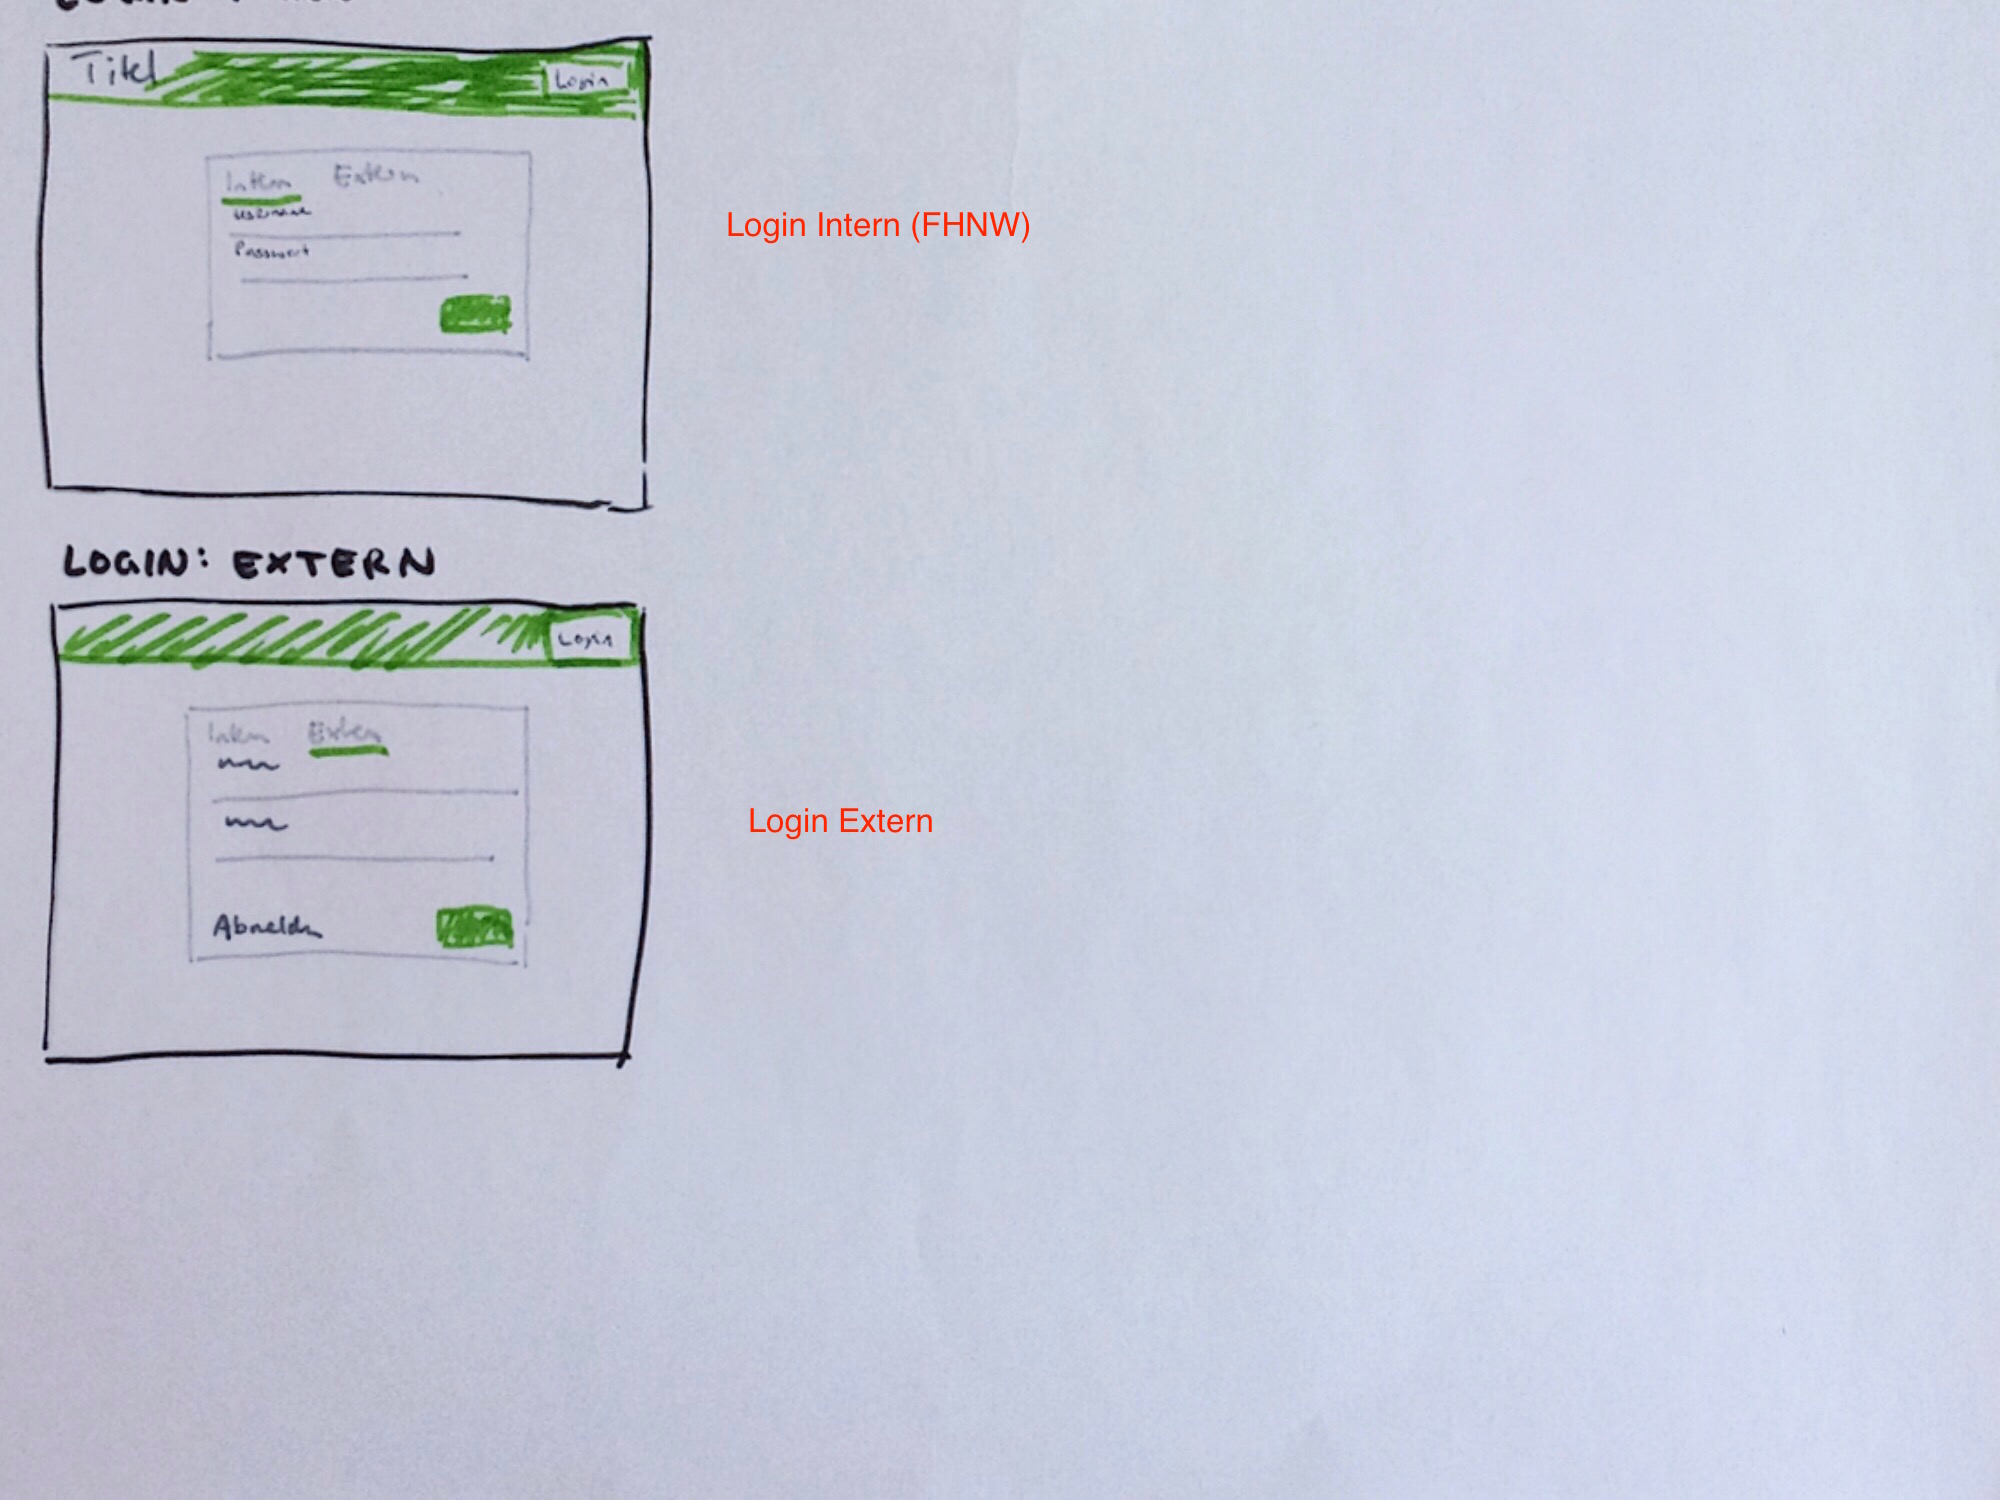
\includegraphics[width=1\textwidth]{prototyp/Login}

\subsection{Übersicht}
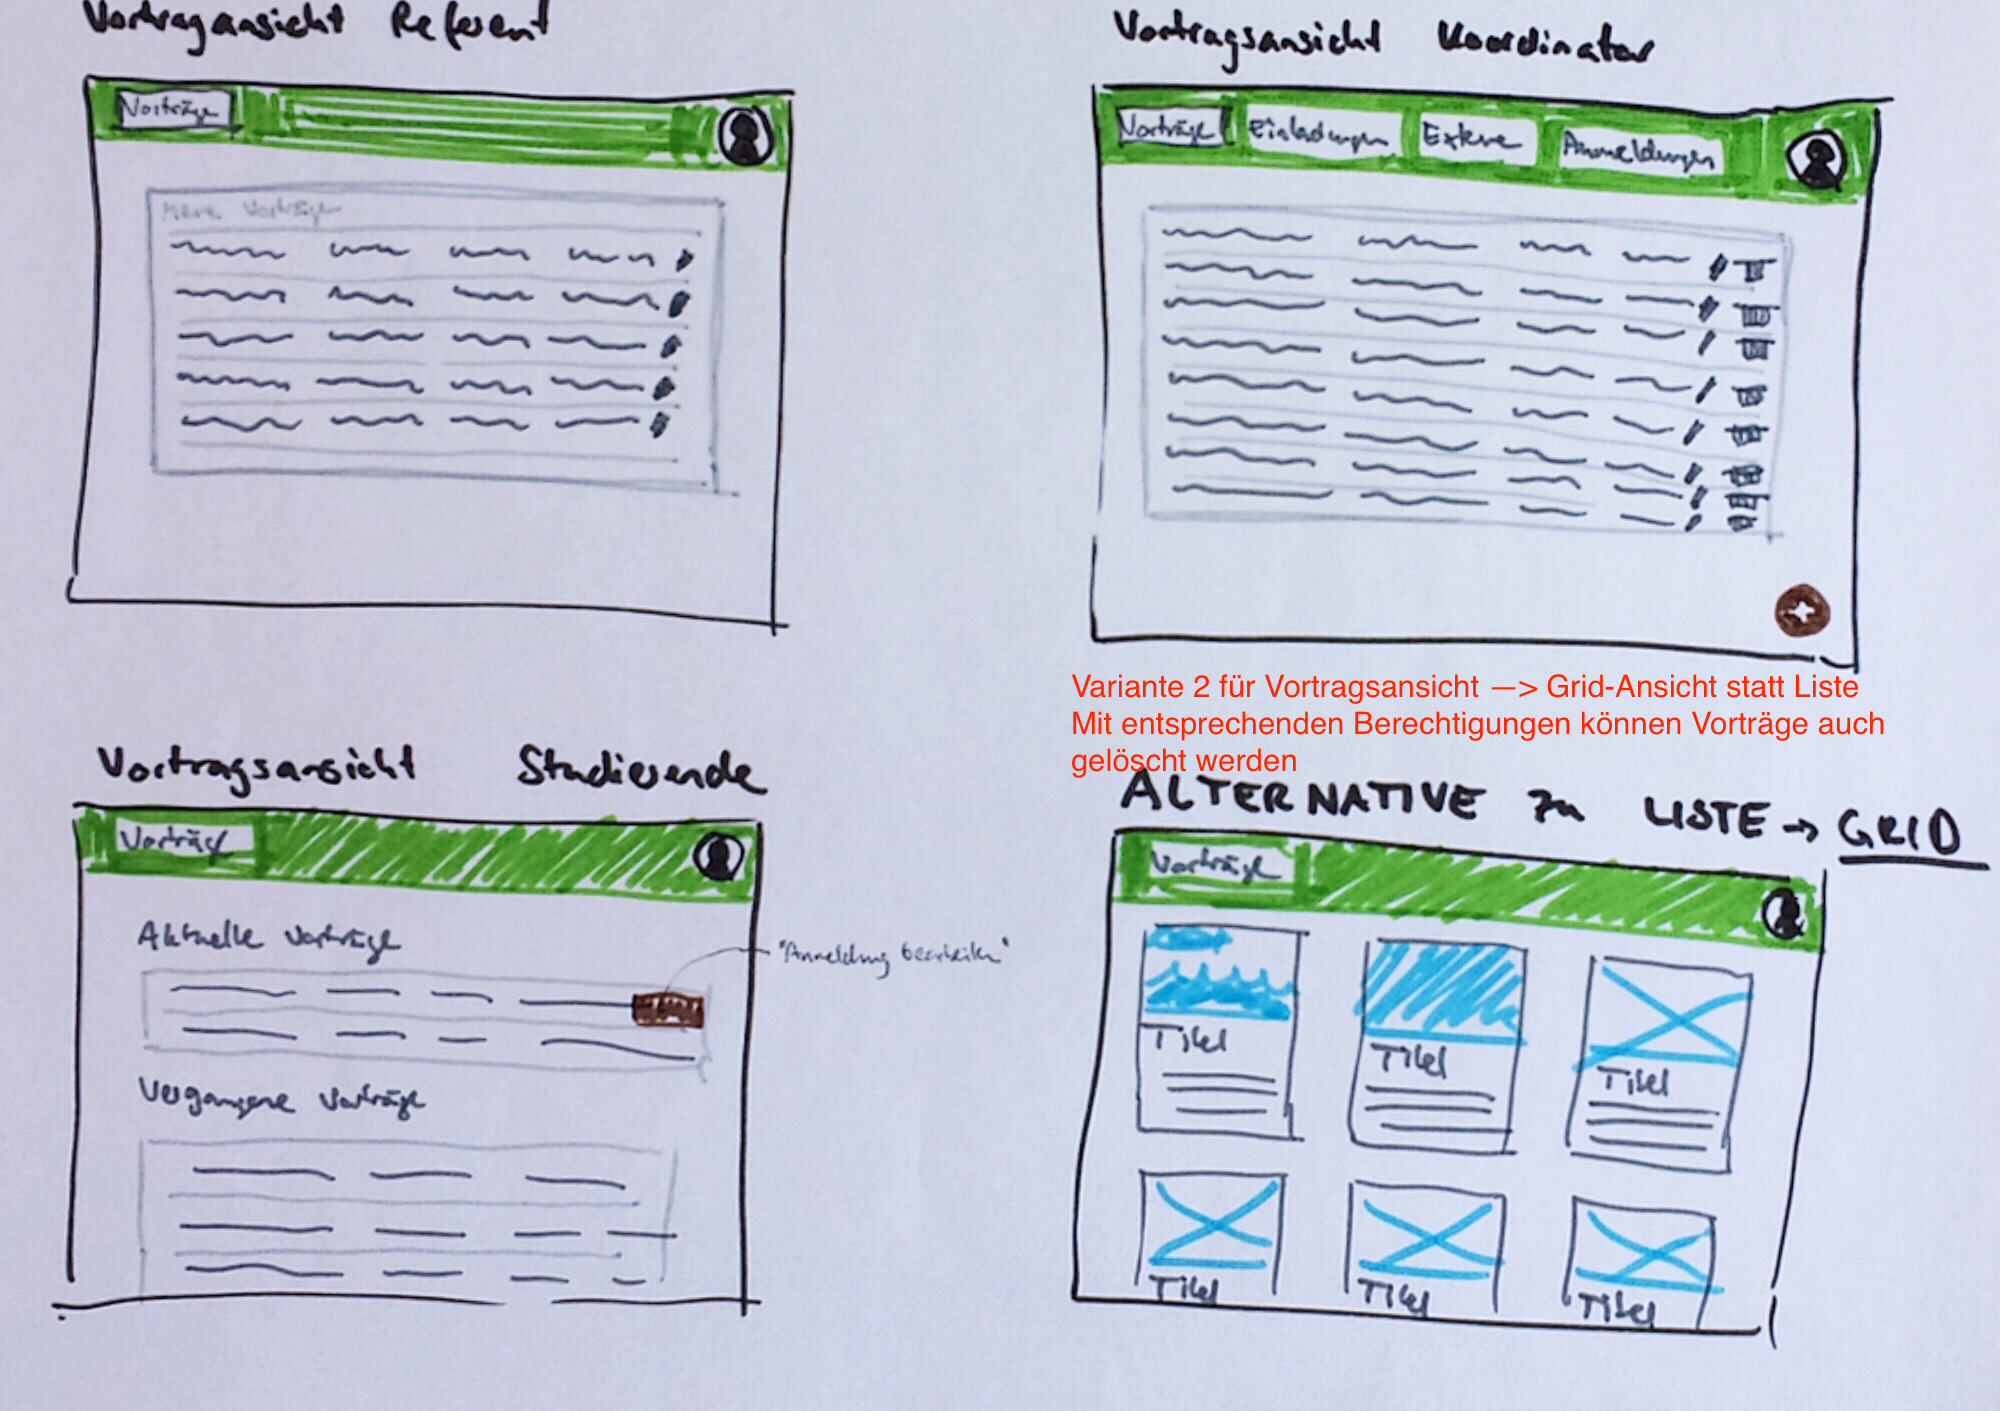
\includegraphics[width=1\textwidth]{prototyp/Vortragansicht}
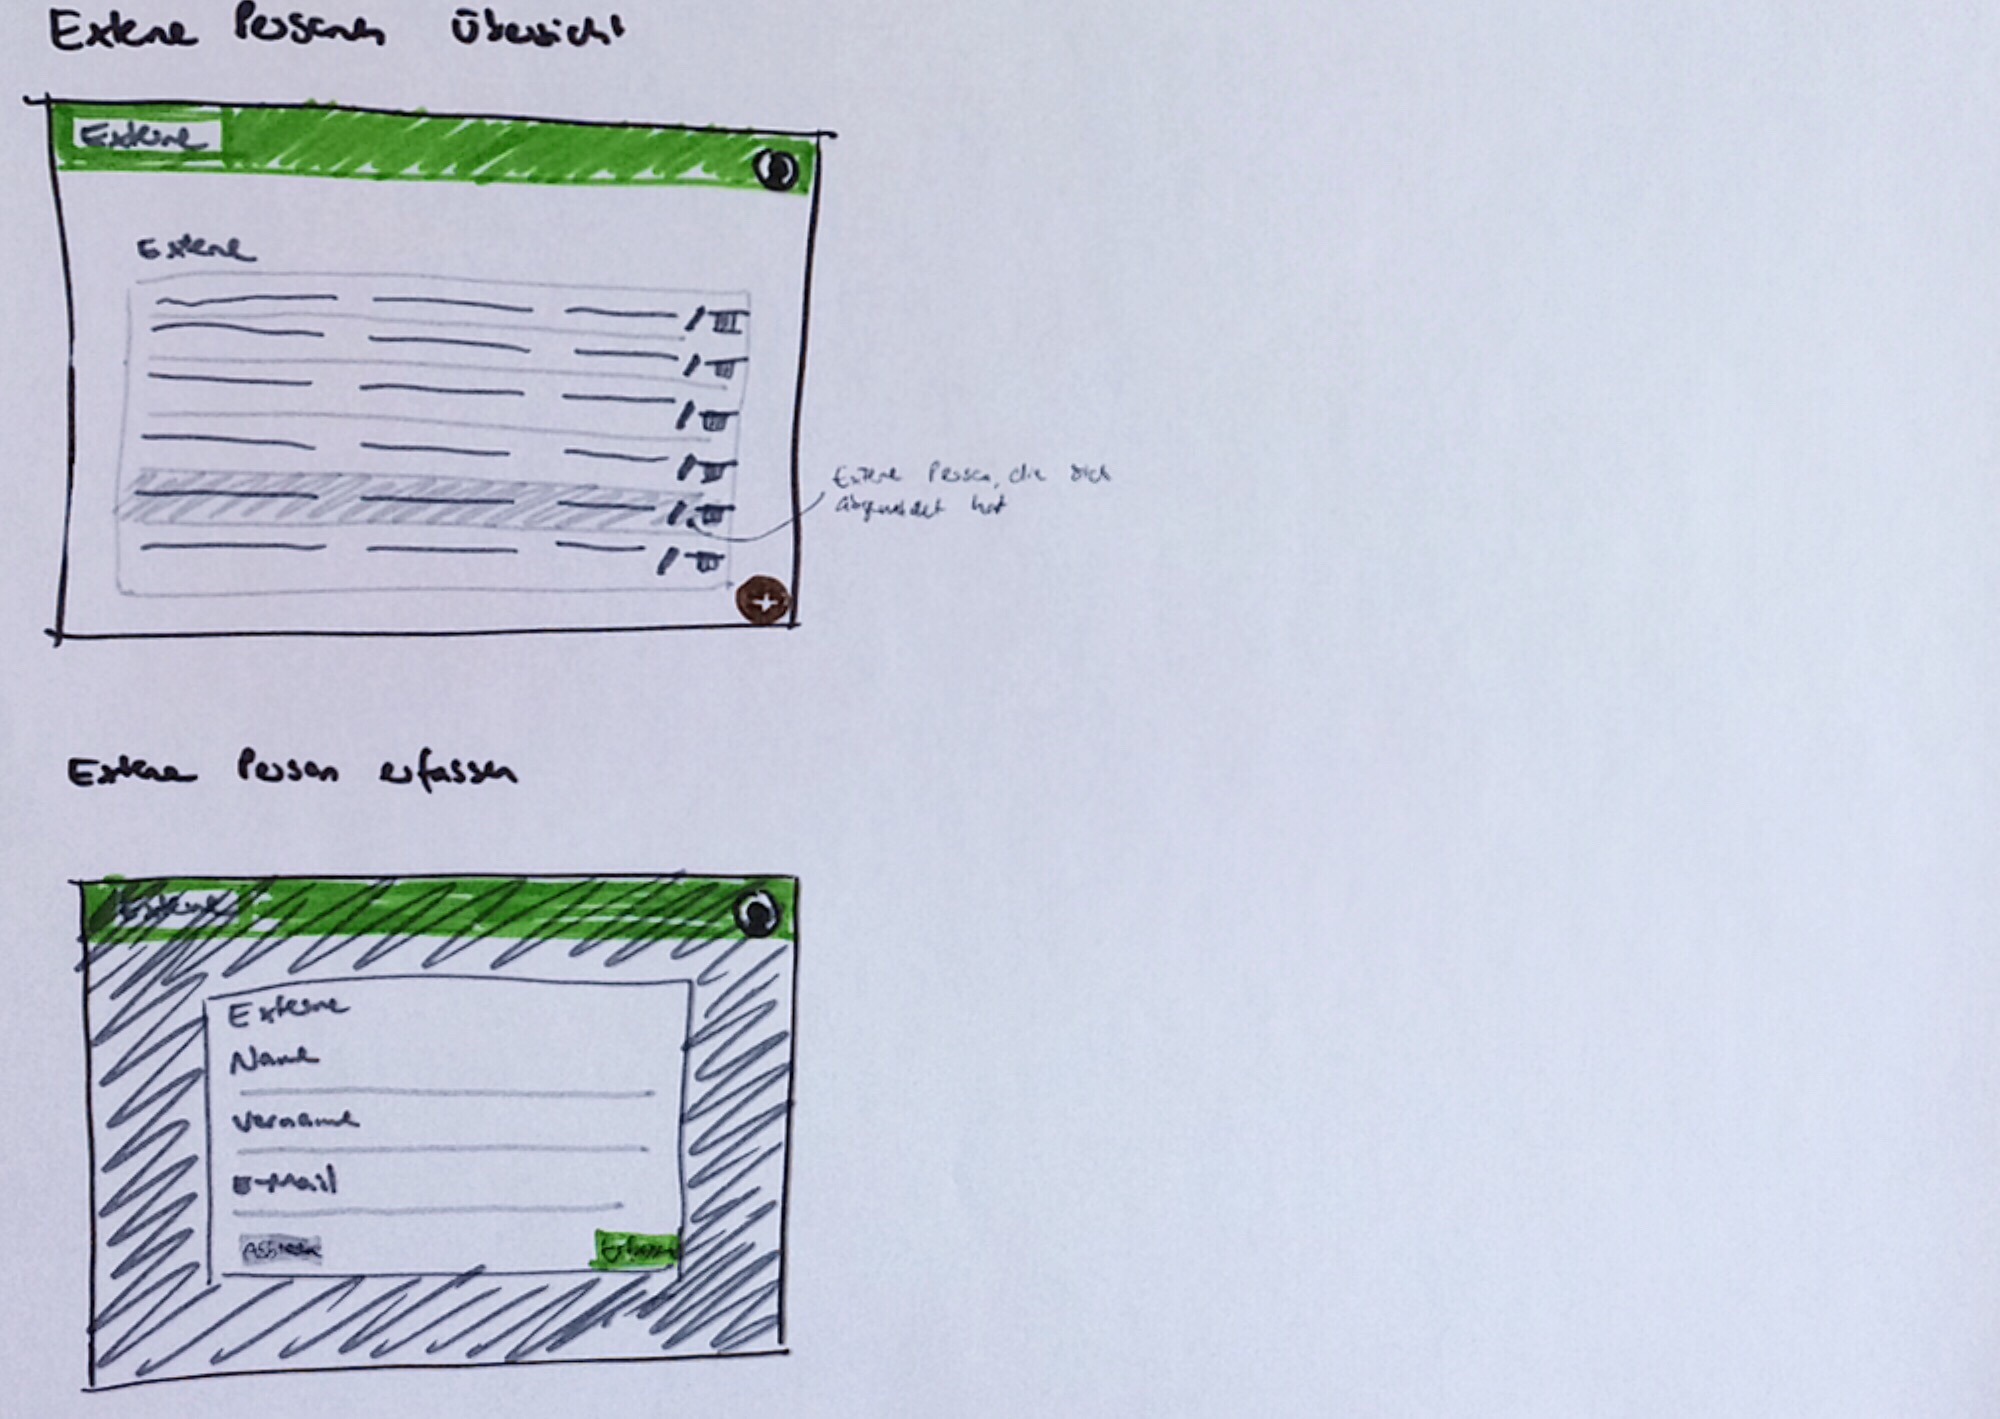
\includegraphics[width=1\textwidth]{prototyp/ExternePersonen}

\subsection{Detailansicht}
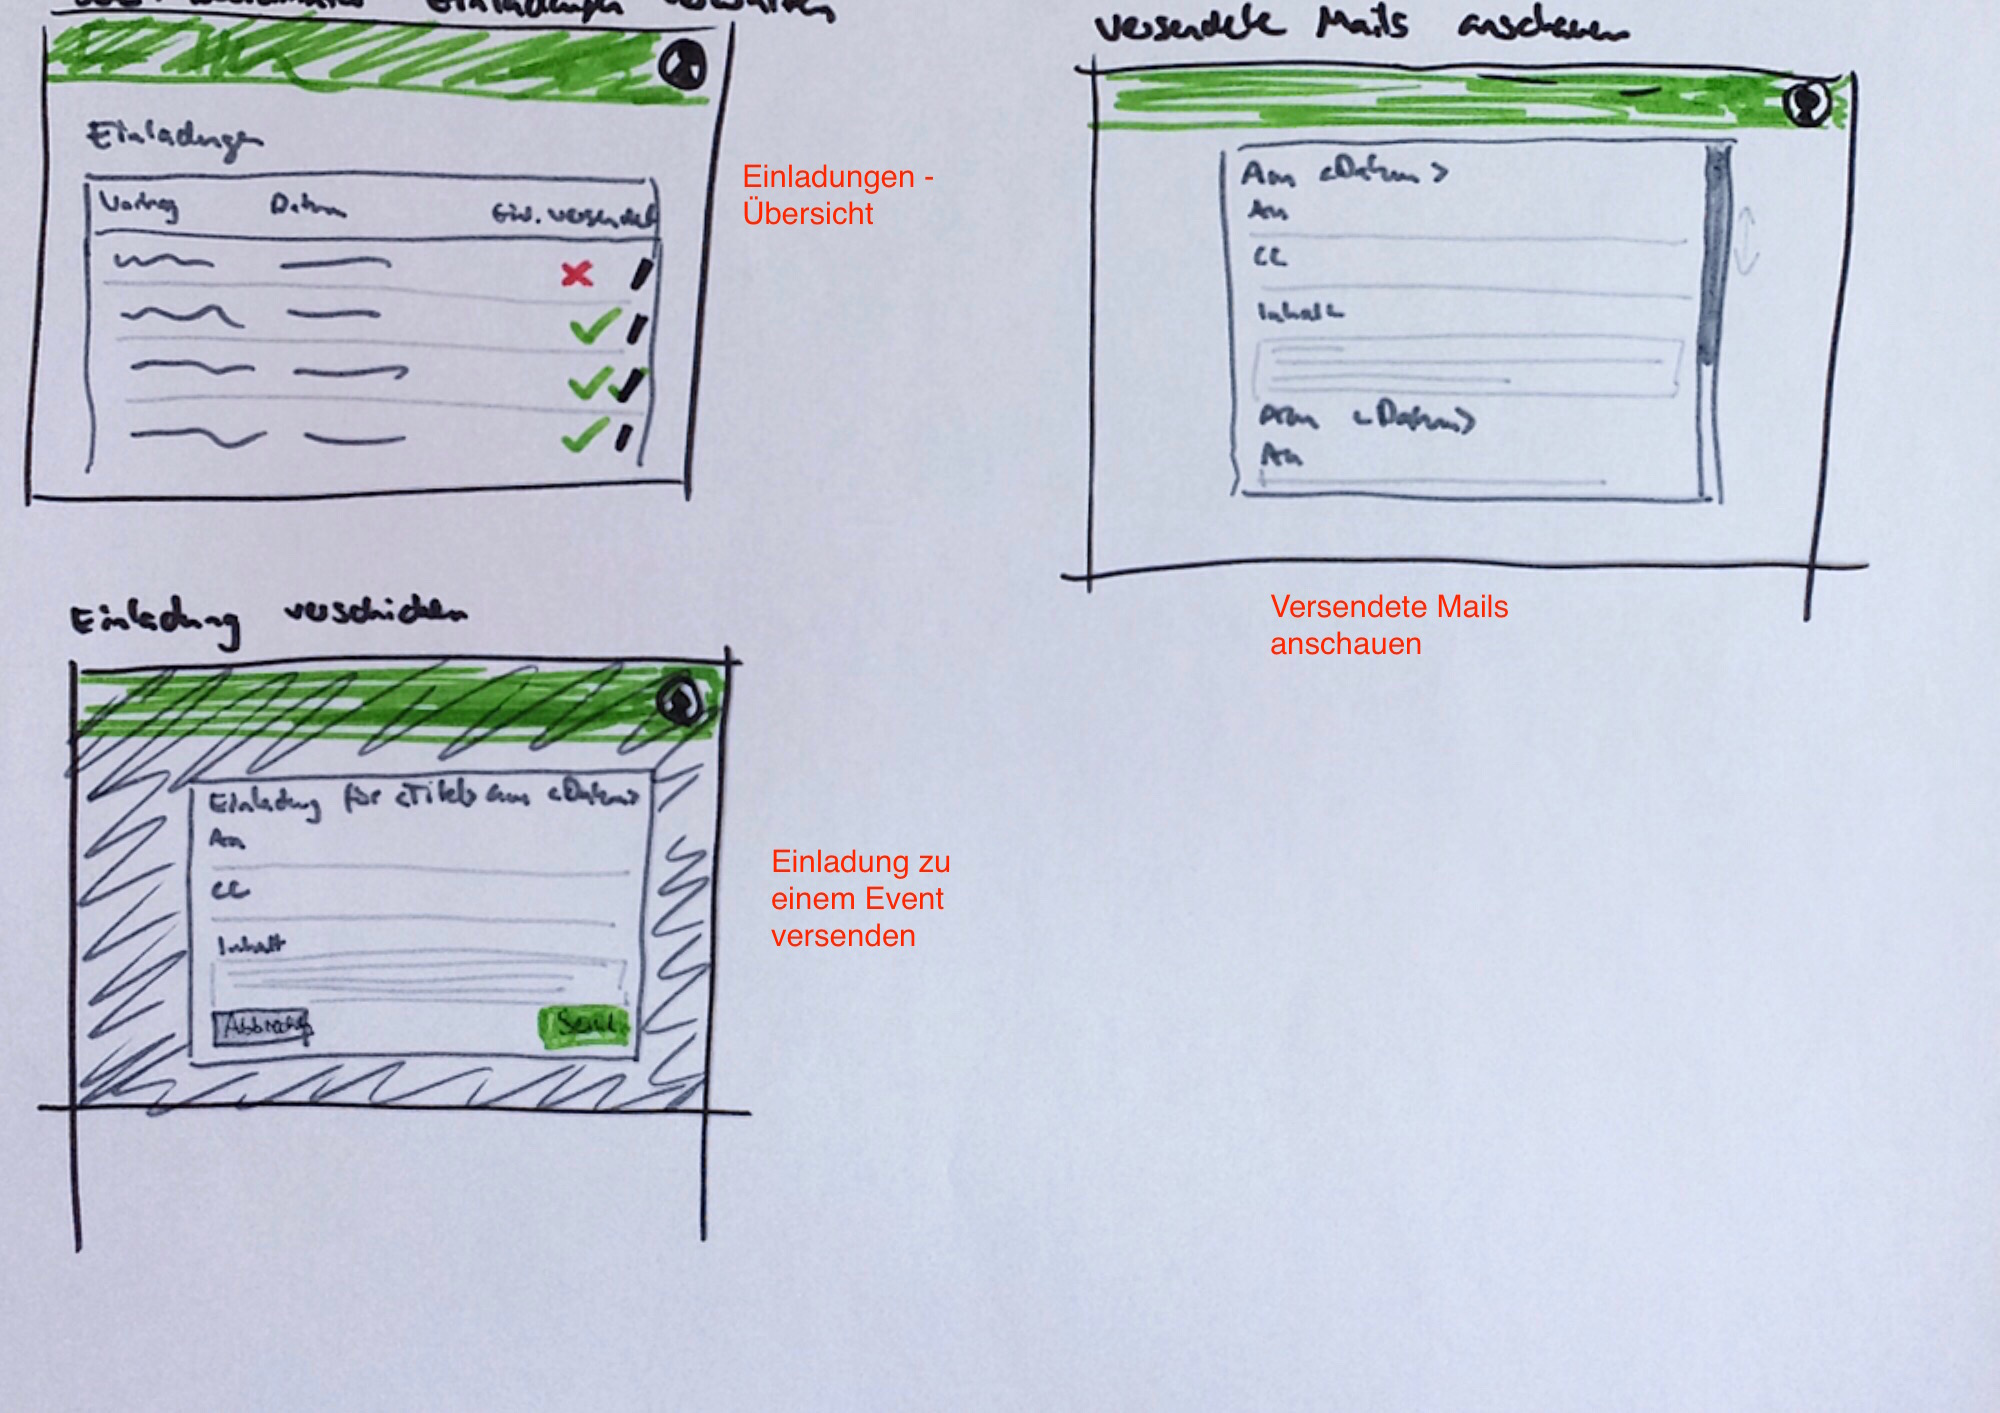
\includegraphics[width=1\textwidth]{prototyp/Einladungen}

\subsection{Einschreiben}
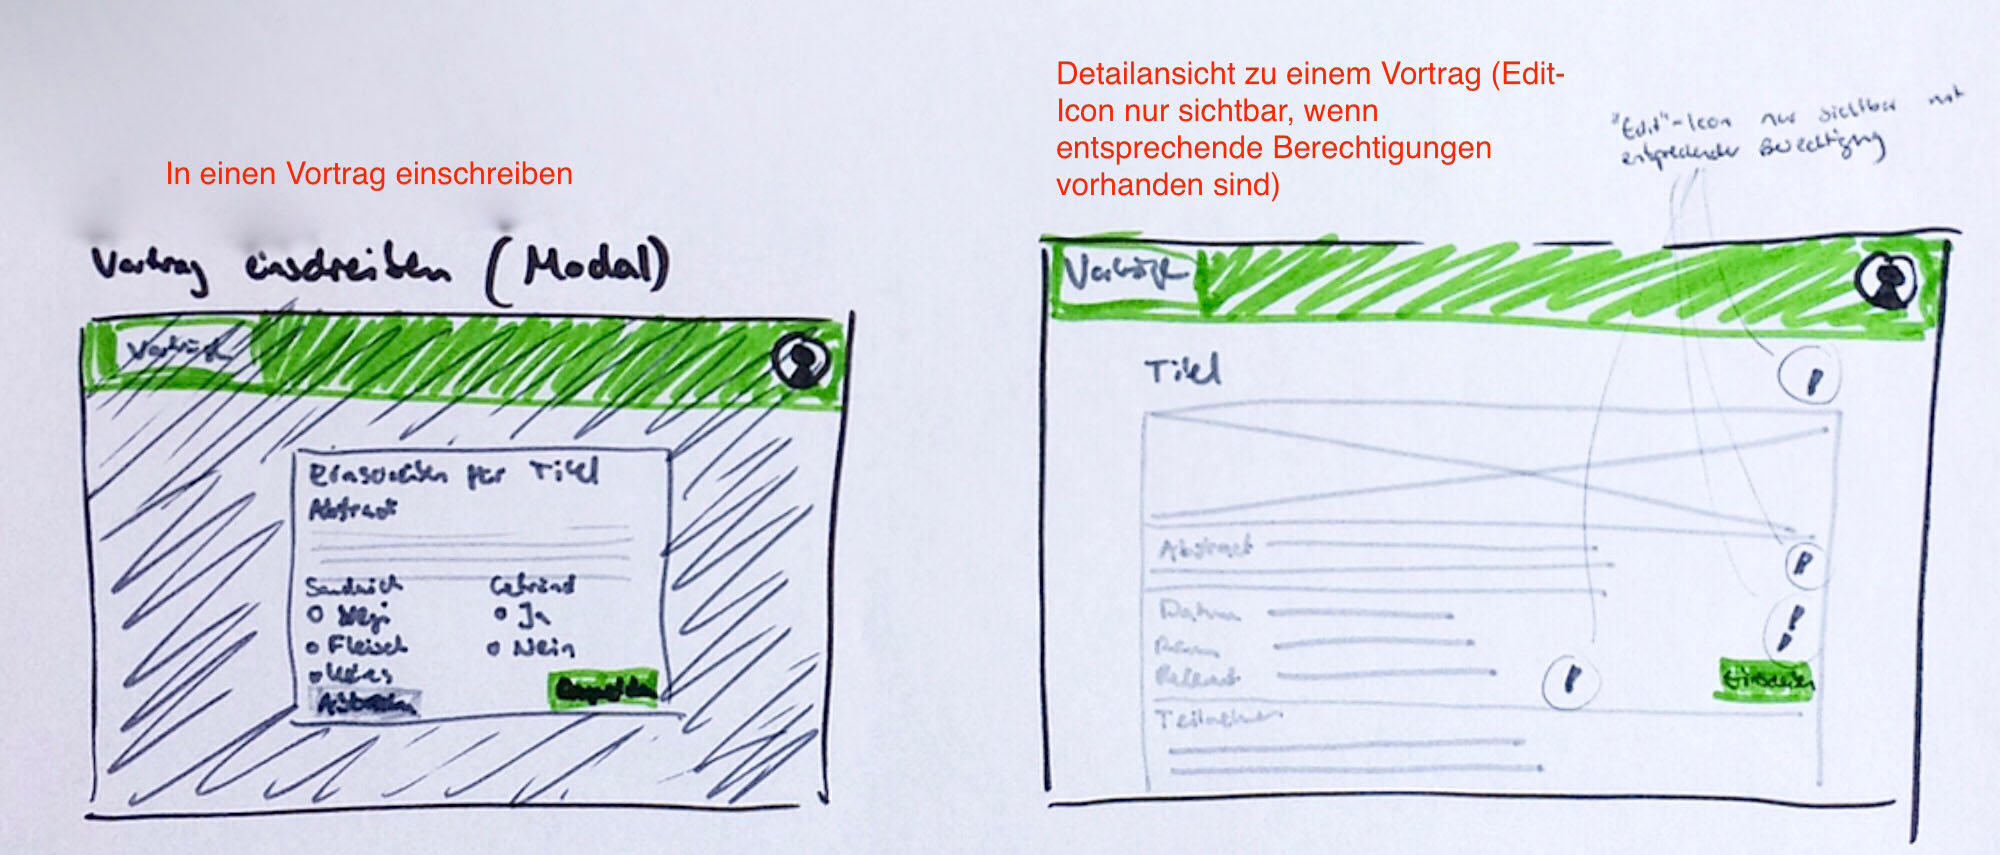
\includegraphics[width=1\textwidth]{prototyp/Vortrag}

\newpage
\section{Architektur - Backend}
Wie bereits in der Einleitung erwähnt, implementierten wir dieses Projekt als Microservices. Wir verwenden dazu "Eureka", eine von Netflix entwickelte Library (siehe auch: https://github.com/netflix/eureka). Die Applikation lässt sich in fünf Microservices unterteilen, welche im nachfolgenden Abschnitt genauer beschrieben werden. Die Microservices kommunizieren ausschliesslich per REST untereinander.

\subsection{Schichtenarchitektur}
\subsubsection{Webschicht}
Die Webschicht wird automatisch durch die einzelnen RepositoryRestResourcen bereitgestellt. Das heisst, die betreffenden RepositoryRestResourcen stellen automatisch die so annotierten JPA-Entitäten via REST-Schnittstelle bereit.

\subsubsection{Businesschicht}
Da das vorliegende Projekt eine relativ einfache Business-Schicht aufweist (vielfach handelt es sich um einfache GET/POST/PUT/DELETE auf bestehenden Entitäten), wird diese meist ebenfalls von den RepositoryRestResourcen wahrgenommen.
Wo eine etwas ausgefeilterte Logik notwendig war wurde diese in der Klasse "CustomPermissionEvaluator" mithilfe von Permissions realisiert. Dabei wird der Zugriff verweigert, sollte die Anfrage von den erwarteten Parametern (z.B. Enddatum vor Startdatum) abweichen.

\subsubsection{Datenbankschicht}
Die Datenbankschicht wurde mit Hilfe von JPA-Repositories realisiert. Für eine Übersicht über das DB-Schema siehe das Unterkapitel Datenbank.

\subsection{Microservices}

Untenstehend sehen wir die Übersicht über unsere Microservicearchitektur:
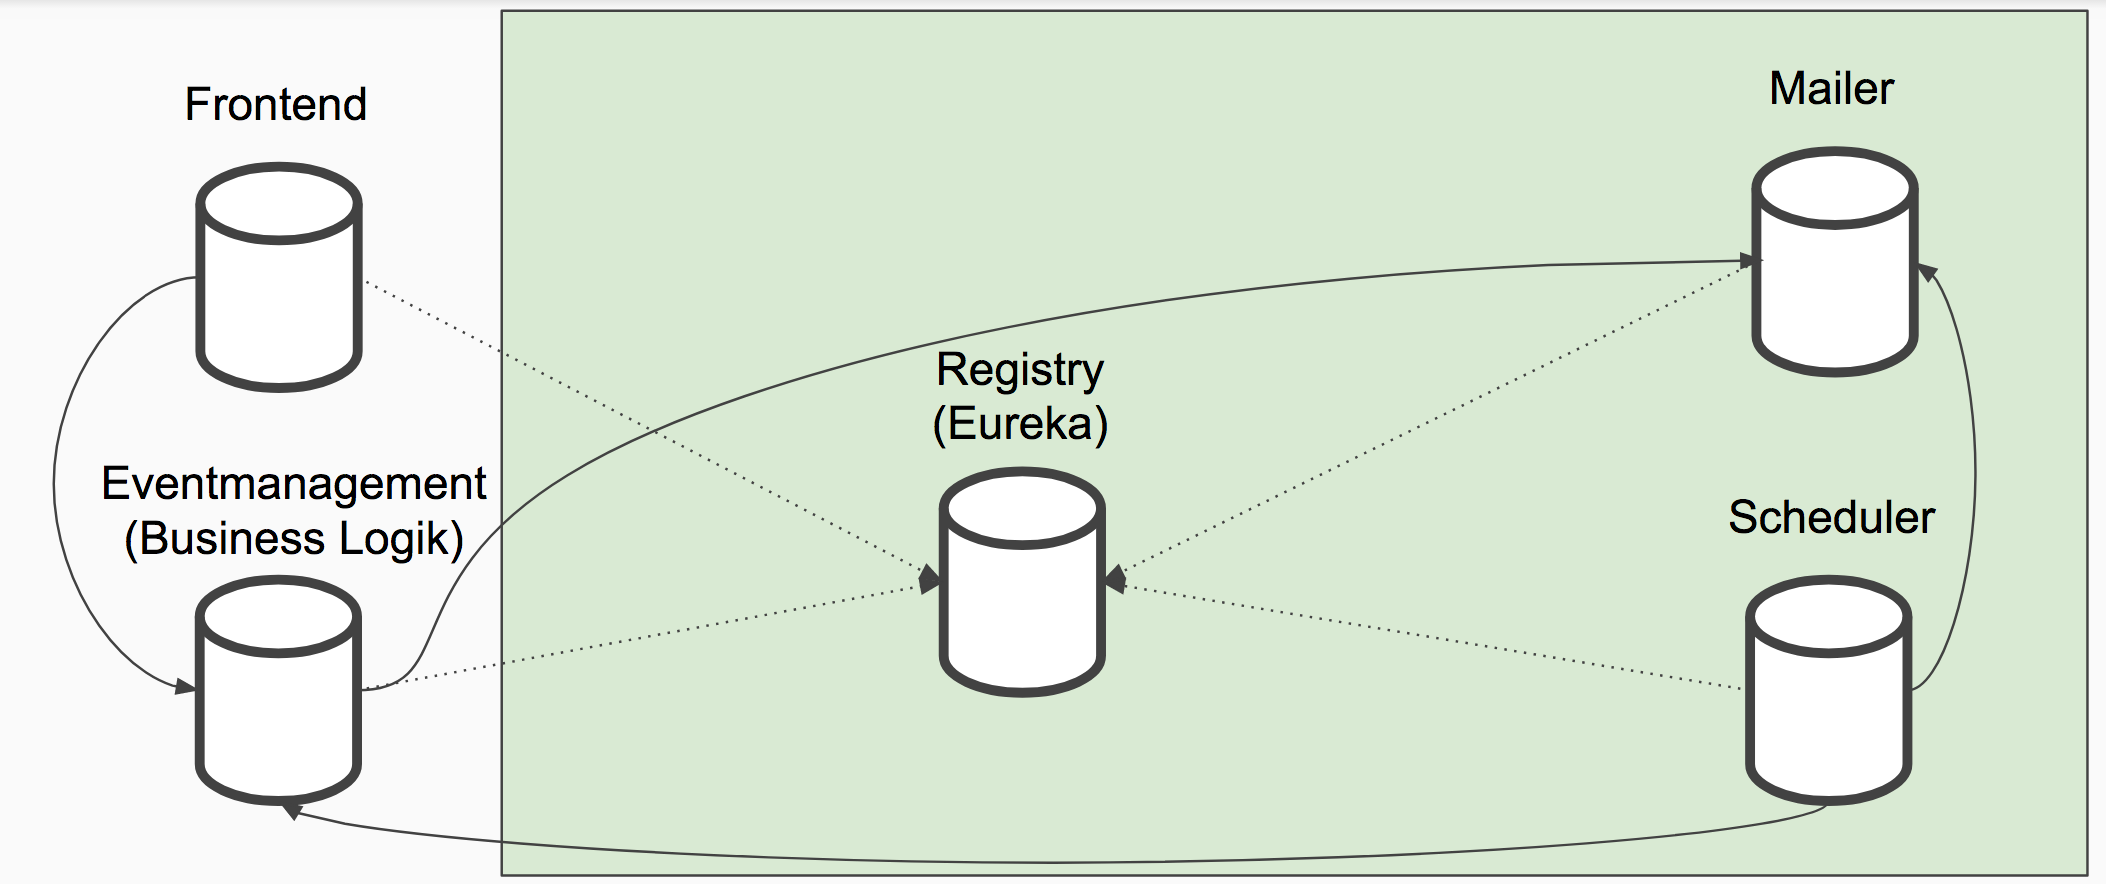
\includegraphics[width=1\textwidth]{microservices}

Die Kommunikation zwischen den einzelnen Services geschieht ausschliesslich über REST. Jeder Microservice meldet sich bei der zentralen Registry (Eureka) an. Im Bild ist ersichtlich, dass ausschliesslich das Frontend und der Eventmanagement Service von ausserhalb erreichbar sind, die restlichen Services sind hinter der Firewall und somit geschützt.

\subsubsection{Registry}
Die Registry stellt das "Bindeglied" zwischen den verschiedenen Microservices dar. Die Microservices verbinden sich auf die Registry um dort die URLs der anderen Microservices zu bekommen. Dadurch wird es möglich die Applikation auf mehreren Servern verteilt laufen zu lassen. Im Falle einer bestehenden Eureka Installation/Architektur muss dieser Microservice nicht nochmals zusätzlich gestartet werden (bestehende Registry kann verwendet werden).
Durch die Verwendung des "Loadbalanced" RestTemplates lösen alle Microservices die logischen Namen anderer Microservices selbstständig mit Rückgriff auf die Registry zu korrekten IP-Adressen auf.

\subsubsection{Eventmanagement}
Der Microservice Eventmanagement ist der zentrale Service unserer Applikation. Er beinhaltet die Persistenzschicht mit allen Entitäten, sowie die Businesslogik der Anwendung. Zudem werden alle Zugriffe auf die Daten und die Logik via diesem Service getätigt. Hierfür werden die CRUD Operationen über eine REST-API zur Verfügung gestellt (mittels den oben erwähnten RepositoryRestResource-Controllern). Bestimmte Endpunkte stehen dabei nur nach erfolgreicher Authentifizierung und Autorisierung zur Verfügung. Die komplette Schnittstellendokumentation ist im Anhang (Swagger Schnittstellendokumentation) aufgeführt.

\subsubsection{Frontend}
Dieser Microservice stellt nur einen Container bereit, der dazu dient, statische Inhalte wie HTML-/CSS-Files, Bilder und so weiter zur Verfügung zu stellen. Er enthält keinerlei Business-Logik und speichert keine Benutzerdaten. Konkret wird der Build Folder unserer Ionic-App in den assets/static Order kopiert. Sollte bereits eine bestehende Webserver Infrastruktur zur Verfügung stehen (z.B. Apache oder Nginx), können diese Assets auch ohne zusätzlichen Microservice gehostet werden.

\subsubsection{Mailer}
Der Mailer ist ein simpler Mailservice, welcher eine API zum Versenden von Mails bietet. Diese API bzw. der Endpoint zum Versenden von Mails wird durch ein statisches Token geschützt, das alle Aufrufer mitschicken müssen, um die zur Verfügung gestellte Funktionalität nutzen zu können. Da der Token nur intern (via application.properties-Files der entsprechenden Microservices) bekannt ist, werden ausschliesslich interne (von anderen Microservices) Anfragen entgegengenommen. Dieser Service ist ein Paradebeispel für einen Microservice, er könnte ohne weiteres für weitere Projekte wiederverwendet werden.

\subsubsection{Scheduler}
Der Scheduler-Service führt zu bestimmten Zeiten verschiedene Tasks aus. Ein Beispiel hierfür wäre, unreferenzierte  Mediendateien in der Nacht zu löschen, Erinnerungsmails zu versenden oder Events aufgrund verschiedener Kriterien zu archivieren.

\newpage
\subsection{Sicherheit}
Die Sicherheit wurde mit von Spring Security und dem Framework Pac4J realisiert. Mithilfe von Pac4J können Permissions und Rollen definiert werden. Abhängig von der Rolle, erhält der Benutzer zusätzliche Privilegien. Ein normaler Besucher kann lediglich Events ansehen und nichts editieren. Wir haben folgende Rollen identifiziert:

\begin{enumerate}
\item Besucher
\item Angemeldeter Gast (kann sich zusätzlich einschreiben)
\item Referent (kann zusätzlich den eigenen Event bearbeiten und Dateien anhängen)
\item Koordinator (kann alle Entitäten bearbeiten und löschen)
\item Service-User (tritt gegen aussen aber nicht in Erscheinung sondern nur, wenn andere Microservices geschützte Dienste des Eventmanagement-Microservice nutzen möchten)
\end{enumerate}

\subsubsection{Rollenkonzept}

Daher haben wir folgende Rollen erstellt:

\begin{enumerate}
\item ANONYMOUS (0) - Besucher
\item REGISTERED (1) - Angemeldeter Benutzer und Referenten
\item ADMINISTRATOR (2) - Koordinator
\item SERVICE (3) - Andere Microservices
\end{enumerate}

Die Rolen sind geordnet und mit Nummern versehen, ein Administrator ist somit automatisch auch ANONYMOUS und REGISTERED. Dadurch lassen sich die Berechtigungen im Frontend bequem realisieren, z.B. sind dadurch Abfragen wie  *ngIf="user.role >= 1" möglich.

\subsection{Authentifizierung}
Zur Authentifizierung stehen zwei Methoden zur Verfügung, wobei das Frontend für den Login Basic Auth und jede weitere Anfrage ein Cookie verwendet. Jede Anfrage kann jedoch auch mit dem Basic Auth gemacht werden (notwendig für Microservices):

\subsubsection{Basic Auth}
Ein bewährter Webstandard, welcher ein Authorization Header mit den encodeten Logindaten verwendet. Serverseitig wird das gefundene Profil in die Session geladen und kann von da an mithilfe des Cookie verwendet werden.

\subsubsection{Cookie}
Nach dem initialen Login mithilfe des Basic Auths, können die Anfragen mit dem Cookie gemacht werden. Das Cookie hat das http only Flag, welches XSS Angrife verhindert (das Cookie kann nicht von Javascript gelesen werden). Beim Logout wird das Cookie gelöscht und ein neues (unautorisiertes) erstellt.

\subsection{CSRF}
Um die Sicherheit zu erhöhen, setzen wir auf CSRF. Bei jeder Anfrage muss ein CSRF Token mitgesendet werden und er Client erhält ein Token für die nächste Anfrage. In unserem Projekt konnten wir alle Endpoints mithilfe von CSRF schützen.

\subsection{CORS}


\newpage
\subsection{Datenbank}
Um für die Datenintegrität garantieren zu können, werden alle Entitäten wie oben durch einen einzigen Microservice verwaltet (https://www.nginx.com/blog/microservices-at-netflix-architectural-best-practices/).
\\
Nachfolgend das Datenbankschema:
\\
\\
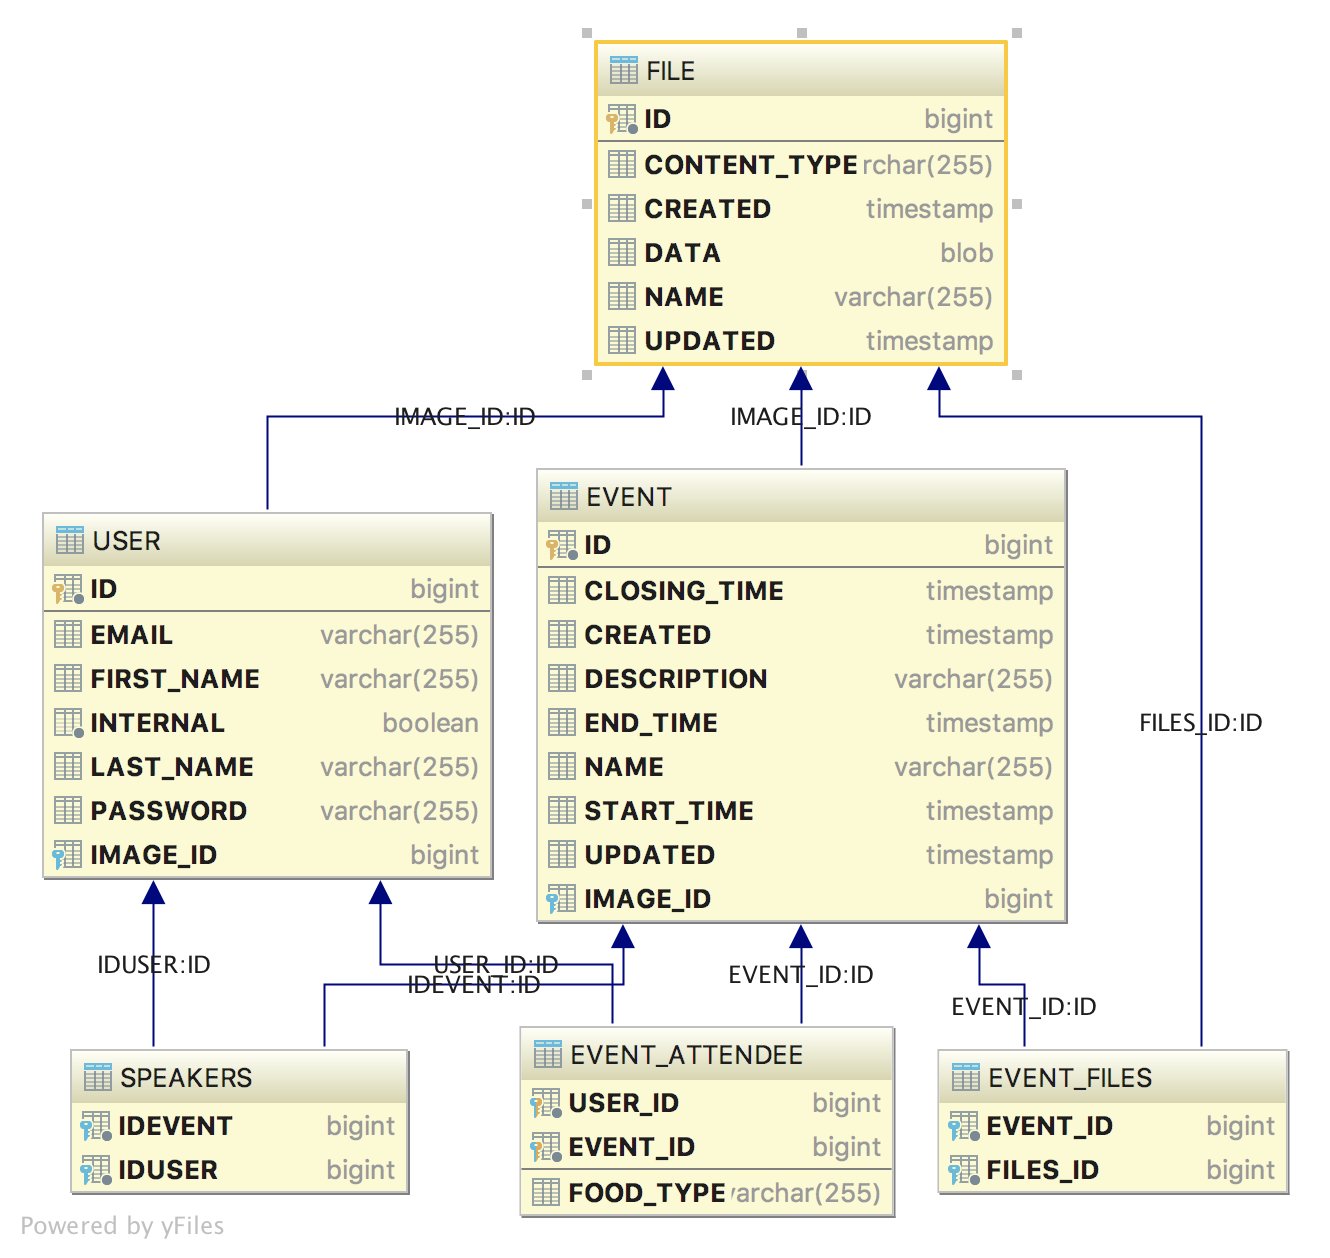
\includegraphics[width=1\textwidth]{dbSchema}
\\

\newpage
\section{Architektur - Frontend}
\subsection{Ionic}
Unsere Ionic app haben wir mithilfe des Ionic CLIs erstellt. Wir sind vom "sidemenu" starter ausgegangen und haben im ersten Schritt die "split-pane" eingebaut, welche der App Standardmässig eine "Desktop-Ansicht" hinzufügt. Lazy loading wurde nicht verwendet, da dies Anfangs noch nicht unterstützt wurde. Da unsere App relativ klein und Übersichtlich ist, besteht sie lediglich aus einem grossen "AppModule", welches alle weiteren Module enthält.

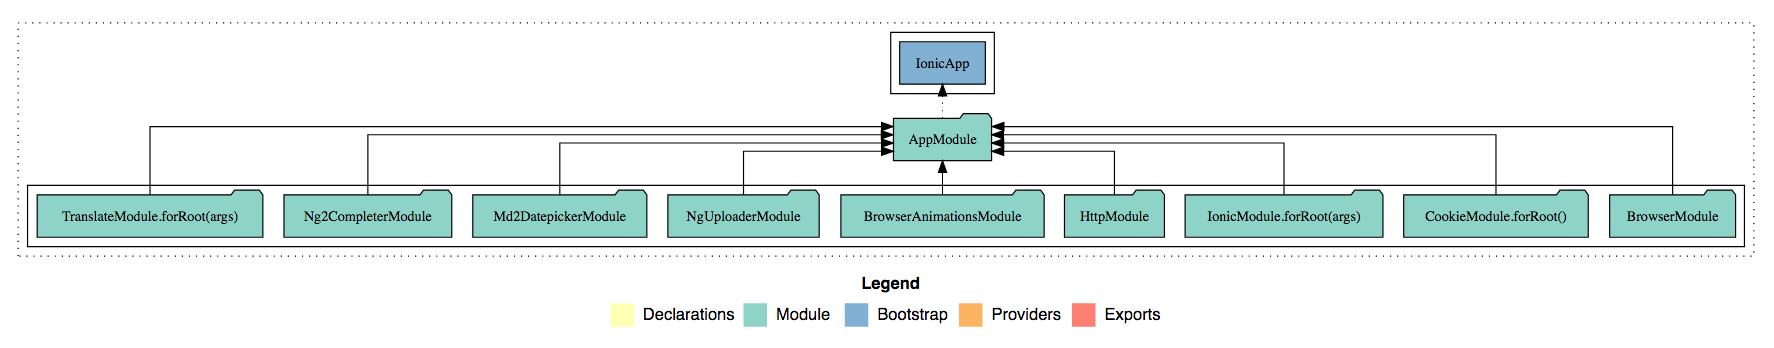
\includegraphics[width=1\textwidth]{ionic-architecture}

Ionic bietet ebenfalls die Möglichkeit, eine Webapp als Progressive Web App (PWA) zu deployen. Dies ermöglicht es in modernen mobilen Browsern auf Funktionen zuzugreifen, die sonst nur für native Applikationen zur Verfügung stehen. Von unserer App wird diese Funktion momentan nicht genutzt, in Zukunft wäre dies aber denkbar (z.B. für Push notifications).

Zudem ist unsere App komplett nach i18n standard auf deutsch und englisch übersetzt.

\subsection{Angular}
Angular bietet ein solides Framework, welches bereits viele Funktionen out-of-the-box unterstützt. Oft wiederkehrende Teile werden als "Components" abgekapselt und sind so in verschiedenen Teilen der Applikation verwendbar. Teile, welche ausschliesslich aus Code bestehen (also ohne view/template), werden als provider abgekapselt. Diese können in andere Komponenten injected werden und so wiederverwendet werden. Dieser Aufbau erlaubt ohne externe Tools eine saubere und übersichtliche Architektur.

\subsection{Typescript}
Typescript, ein typisiertes superset von Javascript, erlaubt das schnellere entwickeln von Javascript durch die eingebaute Typ-sicherheit. Die IDE kann mit IntelliSense Fehler schnell finden und man hat zur Runtime weniger Fehler. Unsere Models konnten wir aus den Entities unseres Backends generieren.

\newpage
\section{Projektaufbau - Backend}
Für alle Microservices wurde jeweils ein eigenes Sub-Projekt erstellt, die jeweils aus einem build-, gradle- und src-Ordner bestehen. Für jeden Microservice existiert ein eigenes build.gradle, das die projektspezifischen Abhängigkeiten enthält.
Der Root-Folder des Gesamtprojektes "wodss" enthält alle Microservices, sowie ein Ordner "ionic", der allen Frontend-Code enthält.
\\
Zudem haben wir vier verschiedene .sh-Files erstellt, mit denen die vier Microservices Eventmanagement, Registry, Mailer und Scheduler je einzeln gestartet werden können. Dazu ein .sh-File mit dem alle erwähnten Services zusammen gestartet (run.sh) werden können, gestoppt werden können (kill.sh) oder gestoppt und gleich neu gestartet werden können (restart.sh). Die einzelnen .sh-Files wurden vor allem während der Entwicklung benötigt, da wir nicht immer alle Microservices miteinander neu starten wollten (da das seine Zeit dauerte), sondern gezielt einzelne Services restarten hochfahren wollten. So konnten Änderungen an einzelnen Diensten schneller getestet werden.
\\
Nachfolgend gehen wir kurz auf den internen Aufbau der einzelnen Microservices ein. Dabei werden wir nur den Aufbau des src-Ordners präsentieren, da sich der Build- und Gradle-Ornder jeweils sehr ähnlich zeigen. Zusätzlich werden auch die relevanten Klassen-Diagramme (in UML) pro Microservice präsentiert.

\subsection{Registry}
Die Registry hat folgende sehr simple Projektstruktur:
\\
\\
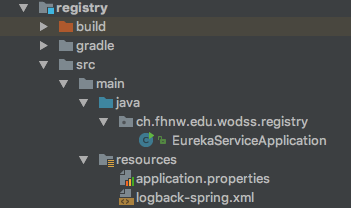
\includegraphics[scale=0.7]{structure_registry}
\\
\\
Der Grund für die schlanke Struktur liegt auf der Hand: da sich die Verwendung der Eureka-Library in diesem Projekt grösstenteils auf Annotationen beschränkt besteht die Registry nur aus einer einzigen Klasse, die mittels "EnableEurekaServer" und "SpringBootApplication" annotiert wurde. Die restlichen Microservices verwenden als Klienten die Annotation "EnableDiscoveryClient".
\\
Das Klassendiagramm präsentiert sich wie folgt:
\\
\\
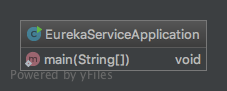
\includegraphics[width=1.0\textwidth]{class-diagrams/Registry-00}
\\
\\
\subsection{Eventmanagement}
Dieser Microservice ist der komplexeste der fünf. Die grobe Struktur präsentiert sich wie folgt:
\\
\\
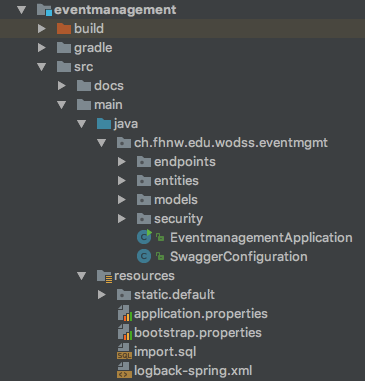
\includegraphics[scale=0.7]{structure_eventmanagement}
\\
\\
Die Swagger-Configuration-Klasse übernimmt, wie der Name erahnen lässt, die Konfiguration der Swagger-Dokumentation der REST-Schnittstelle. Die Klasse Eventmanagement-Application dient der Initialisierung des Microservices. Nachfolgend werden alle Ordner kurz präsentiert und deren Inhalt etwas genauer beschrieben.
\\
Das Klassendiagramm präsentiert sich wie folgt:
\\
\\
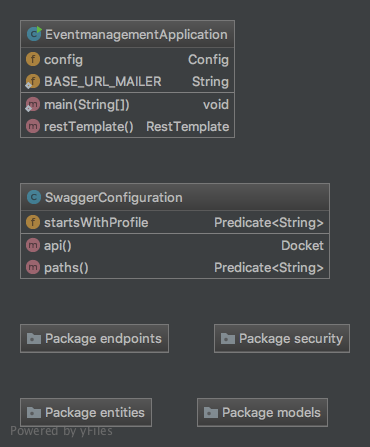
\includegraphics[width=1.0\textwidth]{class-diagrams/Eventmanagement-00}
\\
\\
\subsubsection{Endpoints}
Im Folder "endpoints" sind alle Interfaces und Klassen enthalten, die entweder mittels RepositoryRestResource (sofern die Klasse auf einer konkreten JPA-Entität basiert) oder RestController (sofern die Klasse zusätzliche Geschäftslogik bereitstellt) annotiert sind. Die Struktur sieht folgendermassen aus:
\\
\\
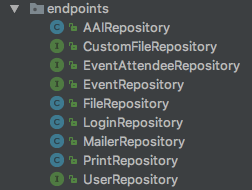
\includegraphics[scale=0.7]{structure_eventmanagement_endpoints}
\\
\\
Relativ schnell erkennt man die zusätzliche Geschäftslogik, die zusätzlich zu den RepositoryRestResource-Controllern programmiert wurde und die nicht durch reine Datenzugriffe verarbeitet werden konnten:
\begin{enumerate}
\item AAI-Repository - verarbeitet Login via Switch-AAI
\item FileRepository - bietet Methoden zum Fileupload und -display
\item LoginRepository - bietet Methoden zum Login und zurücksetzen von Passwörtern
\item MailerRepository - bietet Methoden zum Versenden von Einladungmails
\item PrintRepository - bietet Methoden zum Zugriff auf Druckgerecht-aufbereitete Daten
\end{enumerate}
Die restlichen Interfaces beinhalten zum einen die vom JPA-Repository zur Verfügung gestellten Methoden für den Datenzugriff. Zusätzlich dazu wurden, je nach Bedarf, weitere Methoden für die Datenmanipulation erstellt.
\\
Das Klassendiagramm präsentiert sich wie folgt:
\\
\\
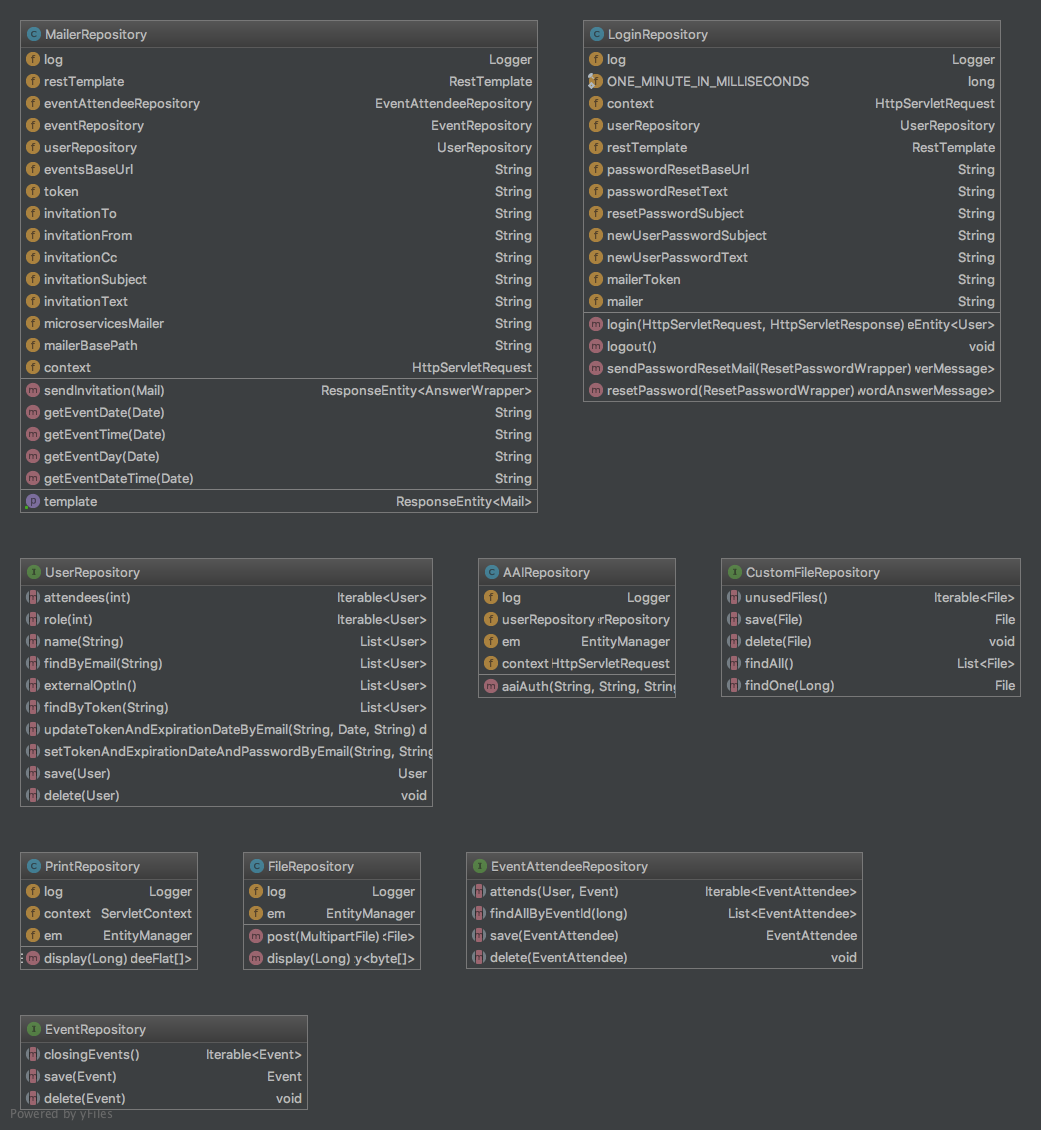
\includegraphics[width=1.0\textwidth]{class-diagrams/Eventmanagement-Endpoints}
\\
\\
\subsubsection{Entities}
Der Ordner "entities" präsentiert sich wie folgt:
\\
\\
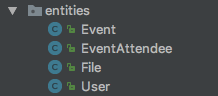
\includegraphics[scale=0.7]{structure_eventmanagement_entities}
\\
\\
Dieser Ordner enthält die tatsächlichen JPA-Entitäten die schlussendlich in der Datenbank als konkrete Tabellen auftauchen (dazu kommen weitere von JPA erstellte Tabellen wie z.B. "Speakers", siehe dazu auch das  Datenkbankschema). Die Entitäten definieren gemäss JPA die verschiedenen Attribute der jeweiligen Objekte.
\\
Das Klassendiagramm präsentiert sich wie folgt:
\\
\\
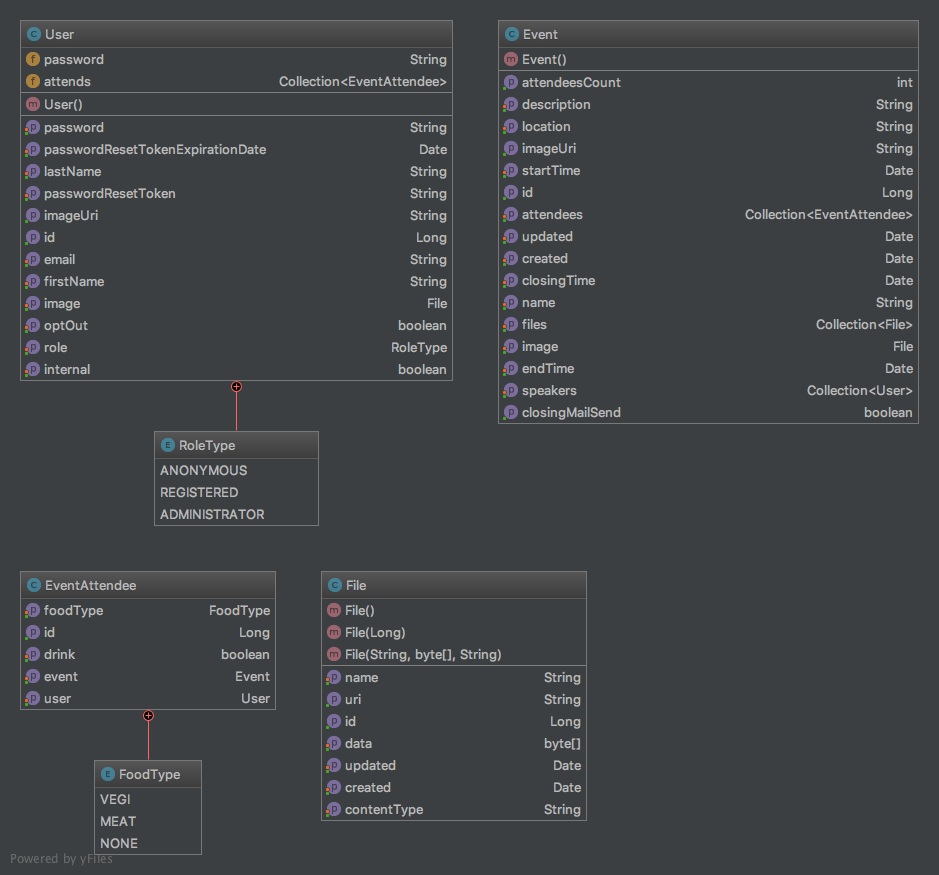
\includegraphics[width=1.0\textwidth]{class-diagrams/Eventmanagement-Entities}
\\
\\
\subsubsection{Models}
Der Folder "model" enhält alle weiteren Objekte, die für das Funktionieren der Applikation notwendig sind, aber nicht persistiert werden sollen:
\\
\\
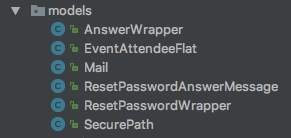
\includegraphics[scale=0.7]{structure_eventmanagement_models}
\\
\\
Eine kurze nähere Beschreibung der verschiedenen Models:
\begin{enumerate}
\item AnswerWrapper
\item EventAttendeeFlat - Container für die druckgerecht aufbereiteten Daten für eine Listenansicht aller EventAttendees (siehe obige Beschreibung des PrintRepository)
\item Mail - Container für den Datenaustausch mit dem Frontend (alles bezüglich Mail) und dem Mailer-Microservice
\item ResetPasswordAnswerMessage - Daten-Container für den Rückgabewert einer ResetPassword-Anfrage (wird im LoginRepository verwendet)
\item ResetPasswordWrapper - Container für die Datenübertragung vom Front- zum Backend während einer ResetPasssword-Anfrage
\item SecurePath - Container der intern verwendet wird, um abgesicherte Pfade zu speichern (wird nur vom CustomizablePathMatcher verwendet)
\end{enumerate} \leavevmode
\\
Das Klassendiagramm präsentiert sich wie folgt:
\\
\\
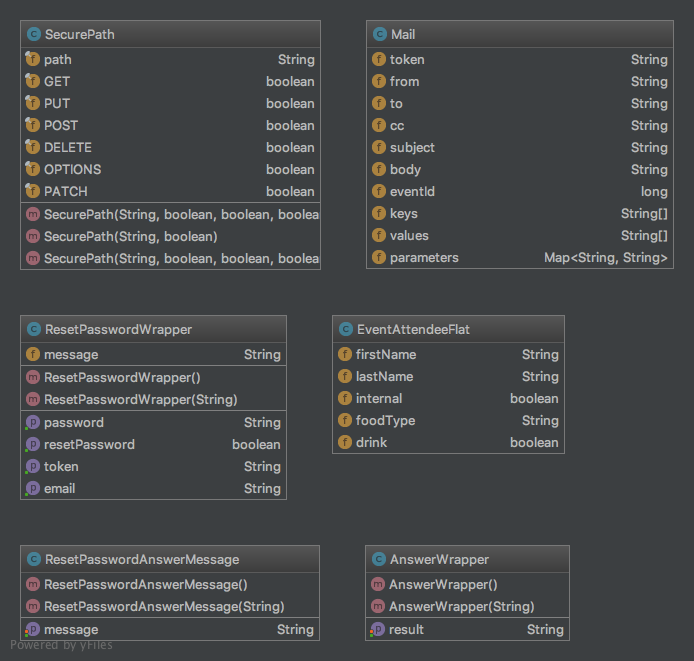
\includegraphics[width=1.0\textwidth]{class-diagrams/Eventmanagement-Models}
\\
\\
\subsubsection{Security}
Der Ordner "security" schlussendlich hat folgenden Inhalt:
\\
\\
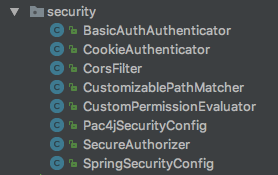
\includegraphics[scale=0.7]{structure_eventmanagement_security}
\\
\\
Eine kurze nähere Erläuterung der verschiedenen Klassen:
\begin{itemize}
\item SpringSecurityConfig - einer der beiden zentralen SecurityConfigs (die andere wäre die Pac4jSecurityConfig). Enthält grundlegende Sicherheitseintstellungen wie z.B. csrf-Schutz
\item Pac4jSecurityConfig - die zweite SecurityConfig. Setzt den CookieAuthenticator, den DirectBasicAuthClient, den Authorizer und legt fest, welche Pfade wie gesichert werden sollen.
\item BasicAuthAuthenticator - verantwortlich für die Authentifizierung via BasicAuth. Verleiht den Usern die ihnen zustehenden Rollen.
\item CookieAuthenticator - validiert einen User anhand eines Cookies, d.h. falls der User bereits eingeloggt ist.
\item SecureAuthorizer - Setzt verschiedene Sicherheitsrelevante HTTP-Header (wie beispielsweise korrekte XSS-Headers usw.)
\item CustomizablePathMatcher - Container für ein Array aus "SecurePaths" (siehe den Unterabschnitt zu "Models"). Matched auf Pfade (wie z.B. /api/login) und gibt die Informationen zurück, welche HTTP-Methoden auf diesen Pfaden erlaubt sind.
\item CustomPermissionEvaluator - bestimmt, ob die korrekten Permissions vorhanden sind, um bestimmte Aktionen auszuführen. Der CustomPermissionEvaluator wird auf den Interfaces im Ordner "Endpoints" aufgerufen, wenn geprüft werden soll, ob ein User die korrekten Permissions hat, um die mit "hasPermission(…)" annotierte Methode auszuführen.
\item CorsFilter - liefert die Funktionalität, um Cors korrekt zu verarbeiten. Wird im vorliegenden Projekt nicht verwendet, da alle Microservices intern gestartet werden bzw. hinter ein und demselben Endpoint (cs.fhnw.technik.ch). Cors stellt somit kein Problem dar. Kann bei Bedarf eingeschaltet werden.
\end{itemize}
\leavevmode \\
Das Klassendiagramm präsentiert sich wie folgt:
\\
\\
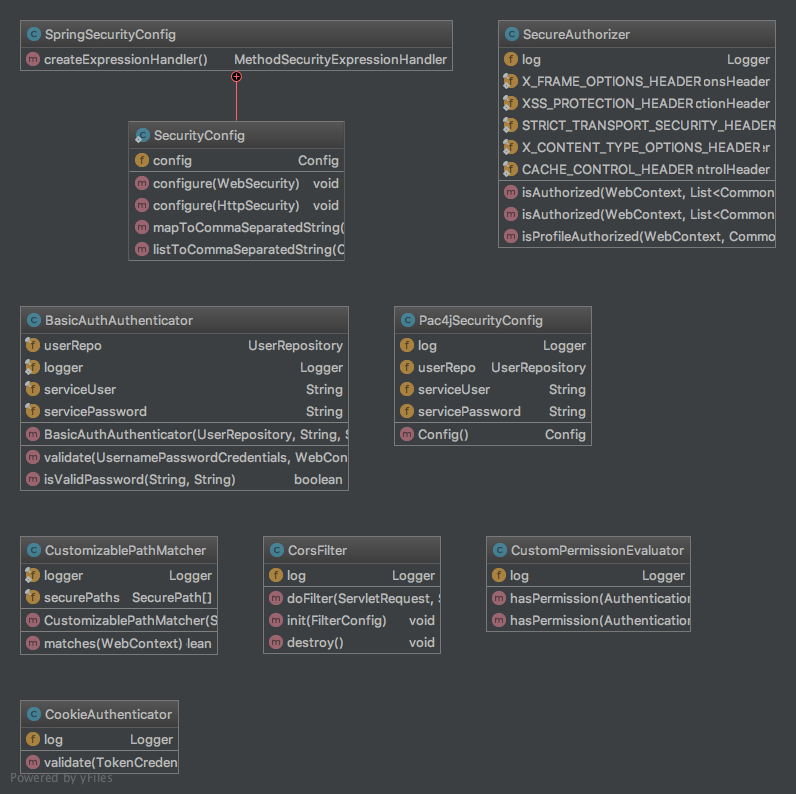
\includegraphics[width=1.0\textwidth]{class-diagrams/Eventmanagement-Security}
\\
\\
\subsection{Frontend}
Der Folder Frontent hält einen relativ bescheidenen Inhalt:
\\
\\
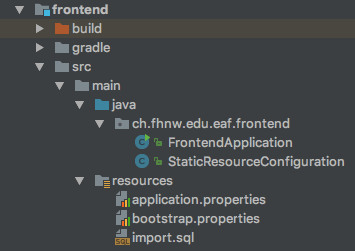
\includegraphics[scale=0.7]{structure_frontend}
\\
\\
Die Klasse FrontendApplication dient dazu, den Microservice zu starten, die Klasse StaticRessourceConfiguration dazu, statische Ressourcen (also die HTML-, Javascript- und CSS-Dateien) auszuliefern.
\\
Das Klassendiagramm präsentiert sich wie folgt:
\\
\\
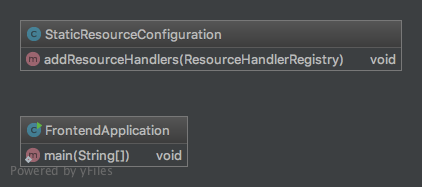
\includegraphics[width=1.0\textwidth]{class-diagrams/Frontend-00}
\\
\\
\subsection{Mailer}
Der Mailer-Microservice ist ebenfalls relativ klein:
\\
\\
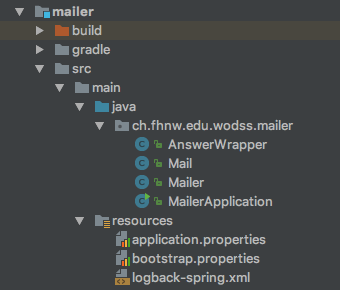
\includegraphics[scale=0.7]{structure_mailer}
\\
\\
Eine kurze Erläuterung dazu:
\begin{itemize}
\item AnswerWrapper - DatenContainer für die Antworten an die aufrufenden Services
\item Mail - DatenContainer für den Input, den die aufrufenden Services an den Mailer schicken
\item Mailer - enthält den zentralen Endpoint für den Mailer (/api/send) an den ein Objekt vom Typ Mail geschickt wird. Das Mail enthält den Text mit eventuellen Platzhaltern und je einem keys- und values-Array mit den Werten, mit denen die Platzhalter ersetzt werden sollen. Der Mailer ersetzt die Platzhalter eigenständig und verschickt das Mail an die im Mail-Container gelieferten Adressen. Er ist somit ein relativ "simpler" Service, der die übergebenen Infos nimmt und mehr oder weniger einfach weiterschickt.
\item MailerApplication - dient dazu, den Microservice zu starten
\end{itemize}
\leavevmode \\
Das Klassendiagramm präsentiert sich wie folgt:
\\
\\
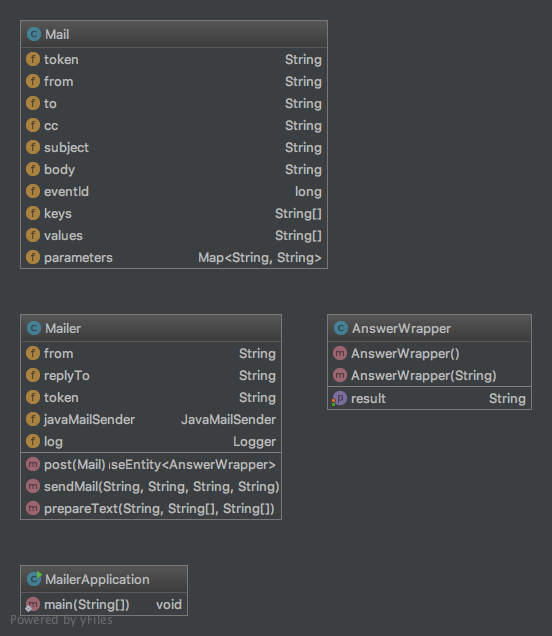
\includegraphics[width=1.0\textwidth]{class-diagrams/Mailer-00}
\\
\\
\subsection{Scheduler}
Der Scheduler-Microservice besteht aus zwei Klassen und einem Unterordner "domain":
\\
\\
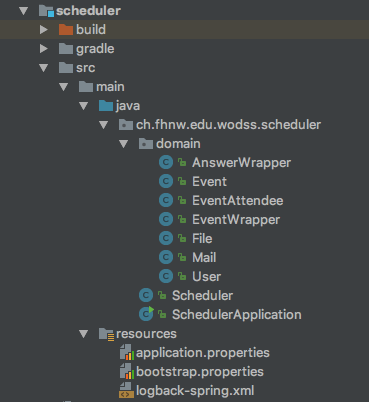
\includegraphics[scale=0.7]{structure_scheduler}
\\
\\
Die SchedulerApplication dient dem Start des Service. Die Klasse "Scheduler" selbst enthält die Logik der Tasks, die in regelmässigen Abständen auszuführen sind.
\\
Das Klassendiagramm präsentiert sich wie folgt:
\\
\\
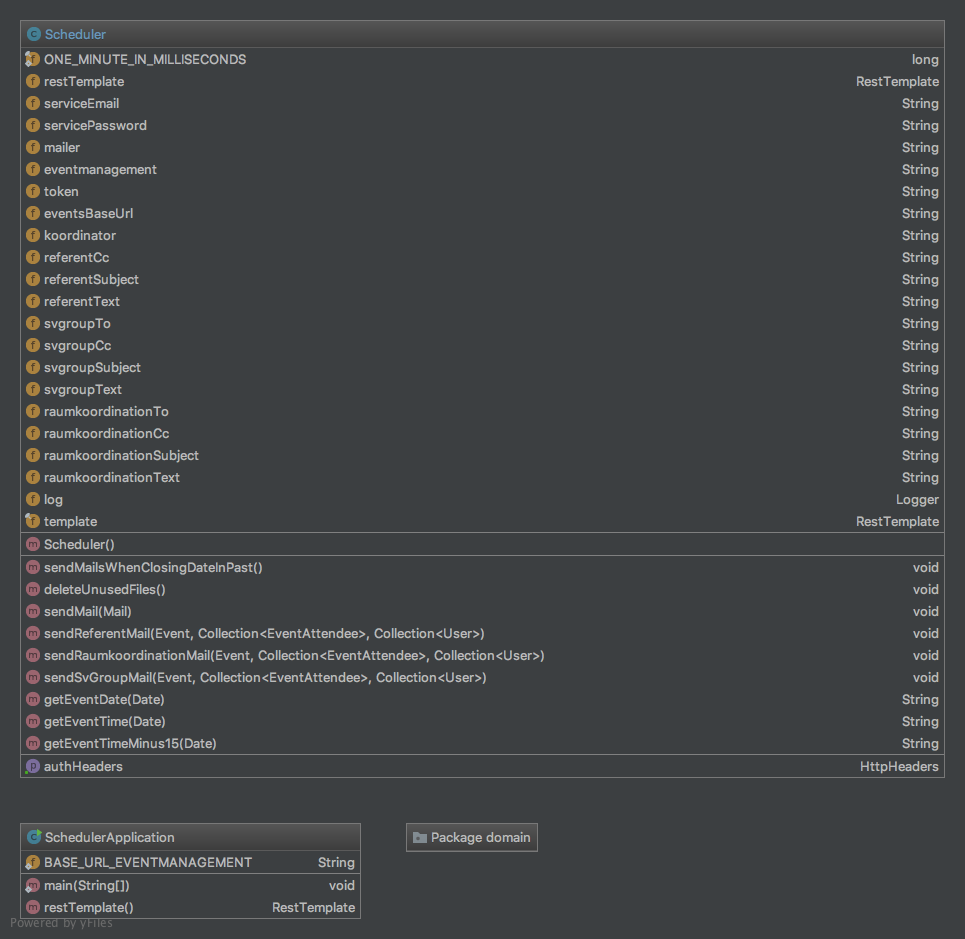
\includegraphics[width=1.0\textwidth]{class-diagrams/Scheduler-00}
\\
\\
Eine kurze Erläuterung des Unterordners "domain":
\begin{itemize}
\item AnswerWrapper - DatenContainer, der bei einem Post auf den Mail-Microservice zurückgeliefert wird. Wird verwendet, um die Antwort auszulesen.
\item Event - Wird verwendet, um die korrekten Daten für regelmässig zu versendende Mails zu erhalten. Die so erhaltenen Informationen werden via keys- und values-String-Arrays innerhalb des Containers "Mail" dem Mailer übergeben (siehe auch Beschreibung des Mailer-Service oben).
\item EventAttendee - Wird ebenfalls verwendet, um die korrekten Daten für regelmässig zu versendende Mails zu erhalten. Die so erhaltenen Informationen werden via keys- und values-String-Arrays innerhalb des Containers "Mail" dem Mailer übergeben (siehe auch Beschreibung des Mailer-Service oben).
\item EventWrapper - DatenContainer der nur jene Attribute eines Events enthält, die in einer "scheduled" Task aktualisiert werden sollen.
\item File - Nimmt dieselbe Funktion ein wie ein Event oder ein EventAttendee (siehe oben).
\item Mail - Container für den Datenaustausch mit dem Mailer-Microservice.
\item User - Nimmt dieselbe Funktion ein wie ein Event, ein EventAttendee oder ein File (siehe oben).
\end{itemize}
\leavevmode \\
Das Klassendiagramm präsentiert sich wie folgt:
\\
\\
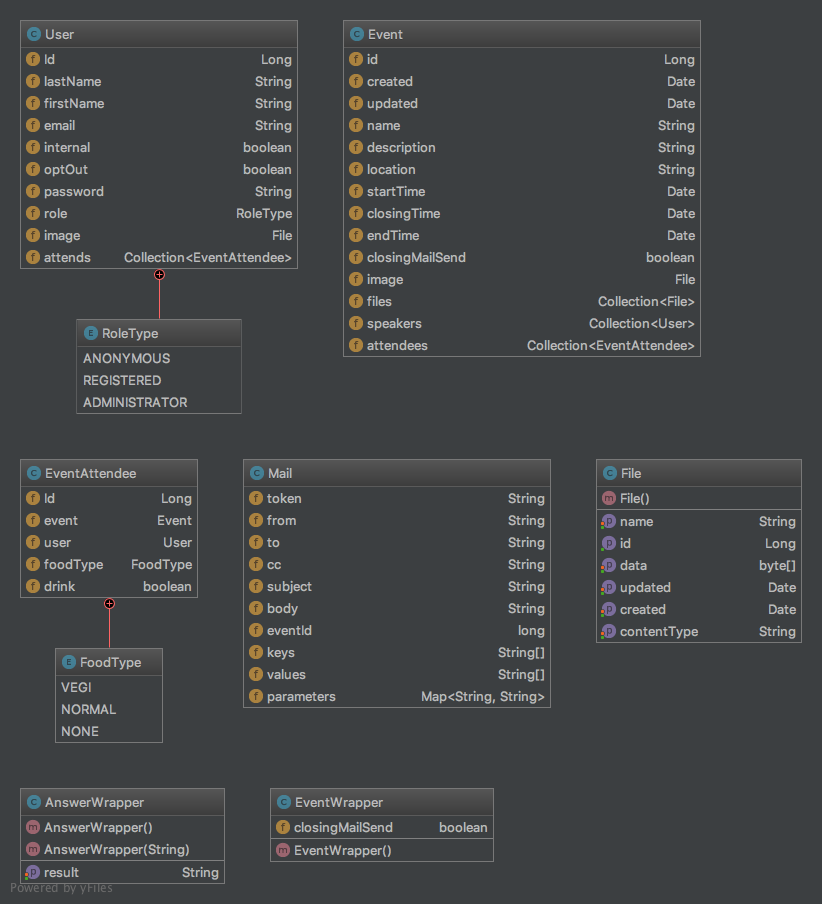
\includegraphics[width=1.0\textwidth]{class-diagrams/Scheduler-domain}
\\
\\


\newpage
\section{Projektaufbau - Frontend}

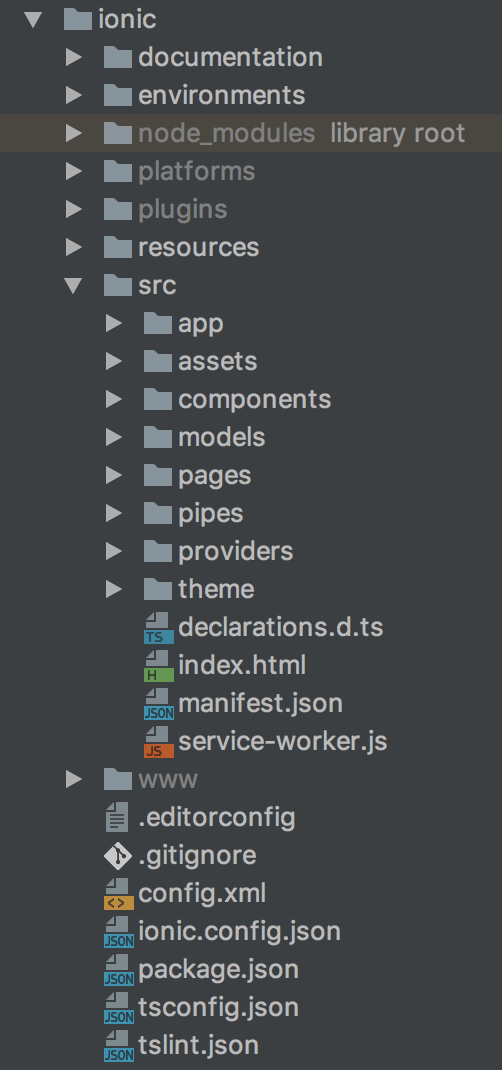
\includegraphics[width=1.0\textwidth]{ionic/ionic-root}
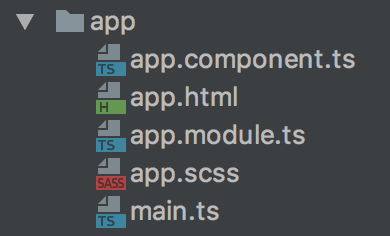
\includegraphics[width=1.0\textwidth]{ionic/src-app}
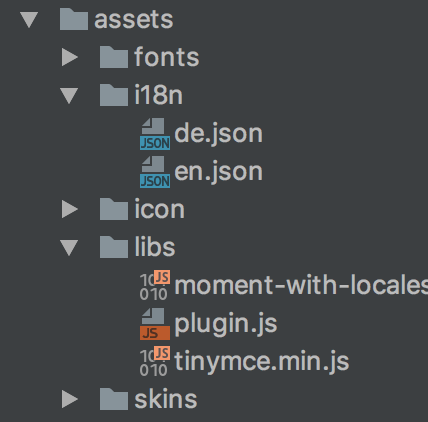
\includegraphics[width=1.0\textwidth]{ionic/src-assets}
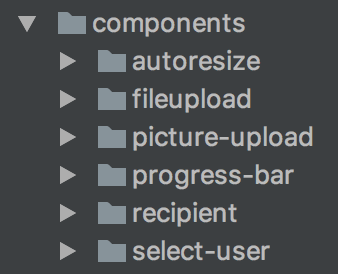
\includegraphics[width=1.0\textwidth]{ionic/src-components}
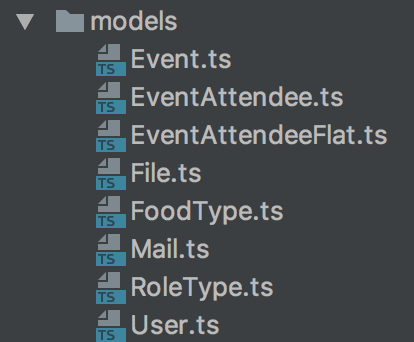
\includegraphics[width=1.0\textwidth]{ionic/src-models}
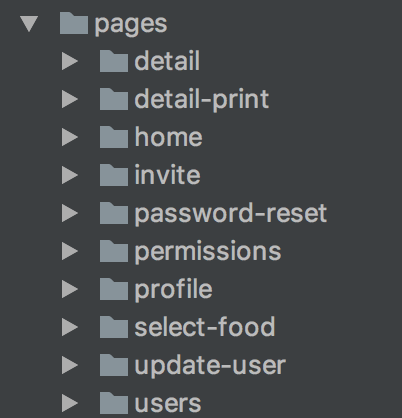
\includegraphics[width=1.0\textwidth]{ionic/src-pages}
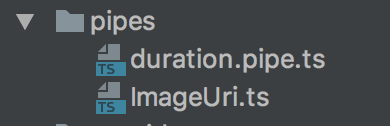
\includegraphics[width=1.0\textwidth]{ionic/src-pipes}
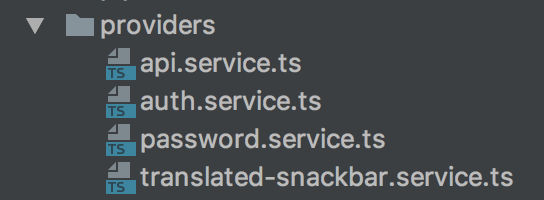
\includegraphics[width=1.0\textwidth]{ionic/src-providers}

\includegraphics[width=1.0\textwidth]{ionic/src-theme}

\newpage
\section{Technologien}

\subsection{Frontend}
Nach dem Start mit Angular 2, entschieden wir uns, das Framework "Angular Material 2" zu verwenden. So wollten wir sicherstellen, dass das Projekt durchgängig eine einheitliche Designsprache verwendet und zudem eine Gestaltung verwendet wird, die aus bekannten Apps (z.B. Google Docs) bereits vielen Usern bekannt sein würde. Das vorliegende Projekt wäre somit inituitiv nutzbar. Relativ schnell realisierten wir, dass "Angular Material 2" aber noch einige Lücken aufwies (beispielswiese fehlten uns einige Standardkomponenten zudem liess die Dokumentation teilweise sehr zu wünschen übrig). Ausserdem war der Aufwand die Seite Mobile-tauglich zu machen grösser als erwartet. Aus diesem Grund wechselten wir nach kurzer Zeit auf Ionic 3. Da Ionic 3 auf Angular 4 aufbaut, war der Wechsel schnell vonstatten gegangen (der Umstieg von Angular 2 zu Angular 4 stellte dabei kein Problem dar). Mithilfe der neuen "Sidemenu-Komponente" konnte die Webseite ohne weitere Probleme für Desktops optimiert werden.
\\
Als Technologien verwendet Ionic 2 wie erwähnt Angular 2 mit Typescript, SASS und HTML.

\subsection{Backend}
Wie von der Projektbeschreibung vorgeschrieben, verwenden wir Java mit Spring Boot im Backend. Zusätzlich verwenden wir die spring-boot-data Erweiterung, welche uns das einfache erstellen von Rest Repositories ermöglicht.
\\
Für den Mailer wurde die Java Mail API, bzw. die Implementierung von Spring Boot verwendet. Um die Informationen in den Platzhaltern von Mailtexten zu ersetzen verwendeten wir die kleine Library "StringTemplate".

\subsubsection{Authentifizierung und Autorisierung}
Für die Authentifizierung verwenden wir Pac4J und Spring Security. 

\newpage
\section{Design-Entscheide}
Anfangs wollten wir verschiedene neue Technologien wie z.B. Elm, GraphQL und Microservices testen. Es stellte sich aber schnell heraus, dass es dabei einige Probleme gibt, welche im folgenden Abschnitt erläutert werden.

\subsection{Microservices}
Wir wählten eine Microservice-Architektur, weil wir dachten, dass wir so die einzelnen Teile relativ unabhängig voneinander gestalten können. Zudem wollten wir diesen Architektur-Typ an einem konkreten Projekt ausprobieren. Es zeigte sich aber, dass eine solche Architektur relativ aufwändig zu erstellen ist: die Schnittstellen zwischen den einzelnen Services müssen genau definiert und gewartet werden. Insbesondere bei einem Refactoring macht sich der zusätzliche Aufwand so bemerkbar: unter Umständen muss man auf mehreren Microservices dieselbe Änderung vornehmen. Weiter zeigt sich, dass sich für das vorliegende Projekt Microservices nicht sehr stark eigenen: die Abhängigkeiten zwischen den verschiedenen Services sind schlicht zu gross (so muss der Scheduler alle Entitätsobjekte des Eventmanagements kennen). Für uns ergibt so schlussendlich einzig der Mailer als Microservice Sinn: dieser ist relativ "stupid" und nimmt nur ein Mail-Objekt entgegen, das anschliessend nach minimaler Verarbeitung versendet wird. So hält sich die Schnittstellen-Definition sehr stark in Grenzen, der Mailer muss keine weiteren Objekte anderer Services kennen und es könnten theoretisch einfach weitere Instanzen des Mailers hochgefahren werden, wenn z.B. sehr viele Mails versendet werden müssten und eine einzelne Instanz an ihre Grenzen gelangt.

\subsection{Security}
Als "Sicherheits-Framework" wählten wir, zusätzlich zu Spring Security Pac4J. Wir wählten Pac4J da es uns eine Authentifizierung via BasicAuth, Cookies, ein simples Route-Matching und einfach zu verwendende XSS-Schutz usw. erlaubt. Ursprünglich planten wir, den CSRF-Schutz ebenfalls über Pac4J zu erstellen. Da Spring Security diese Funktionalität aber auch bietet und wir Probleme beim "einstellen" des CSRF-Schutzes via Pac4J hatten, nutzten wir Spring Security für den CSRF-Schutz. Sehr hilfreich ist ausserdem das Rollen und Permission Model, welches wir auch dazu verwendet haben, die Businesslogik umzusetzen.

\subsection{Ionic}
Wie bereits erwähnten, wählten wir anstelle von Angular Material 2 Ionic 2. Dies taten wir einerseits, da es uns mit Typescript eine sehr willkommene Typsicherheit im Frontend bietet und andererseits, da es mit Ionic Desktop nun auch für "konventionelle" Webprojekte wie das vorliegende hervorragend eignet. Dank den vordefinierten Komponenten konnten wir so einige Enticklungszeit im Frontend sparen, die wir statt dessen in andere Teile der Applikation investieren konnten.

\subsection{Elm}
Elm ist eine relativ neue funktionale Sprache, die zu Javascript kompiliert. Der grosse Vorteil von Elm sind die Typsicherheit sowie der funktionale Aspekt. Es sollte dadurch beispielsweise keine Runtime-Fehler, die in Javascript an der tagesordnung sind, mehr geben.
Es hat sich aber herausgestellt, dass das Ökosystem zwar bereits viele Funktionen bietet, wenn man aber genaue Anforderungen hat muss man teilweise Kompromisse eingehen.
Weiter wäre unser Projekt durch die Wahl einer "neuen" Programmiersprache weniger wartbar geworden. Am Ende verzichteten wir deshalb auf Elm als Programmiersprache und wählten, wie bereits erwähnt, Angular 2.

\subsection{GraphQL}
Durch die JPA-GraphQL ist das initiale Aufsetzen eines GraphQL Endpoints nach einigen Versuchen relativ gut gegangen. Leider fehlen der Library aber noch einige zentrale Features, weshalb man nicht komplett auf die REST-API hätte verzichten können. Anstelle von zwei verschiedenen Endpunkten haben wir uns schlussendlich aus gründen der Wartbarkeit für eine "reine" REST-Lösung entschieden.

\newpage
\section{Lessons learned}
Im Laufe unseres Projekts wurden wir mit einigen Problemen konfrontiert, die insgesamt einen grossen Teil unserer Zeit in Anspruch genommen haben.

\subsection{Microservices}
Zu Beginn des Projekts schienen Microservices eine sehr gute Architektur für das Projekt zu bieten. Initial planten wir separate Services für User, Events, Mailer, Scheduler und Frontend zu erstellen. Diese Idee scheiterte aber an der engen Abhängigkeit von User und Events, so wurden diese zwei Entitäten schlussendlich in einem Microservice kombiniert, der zum Schluss im Service "Eventmanagement" resultierte.
\\
Unser Fazit über das gesamt Projekt fällt allerdings durchzogen aus (siehe auch Punkt Design-Entscheide). Als vorteilhaft sehen wir, dass beispielsweise vom Mailer, da er komplett "stateless" ist, beliebig viele Instanzen hochgefahren und genutzt werden können. Vorstellbar wäre z.B. dass ein Mailer-Loadbalancer erstellt wird und nach Bedarf zusätzliche Mailer-Instanzen hochfährt.
\\
Je länger das Projekt dauerte, desto mehr wurden aber auch die Nachteile von Microservices sichtbar: die Schnittstellen zwischen den verschiedenen Services müssen extrem gut definiert werden und ziehen Abhängigkeiten mit sich, die teilweise so zu Beginn nicht sichtbar sind. Beispielsweise muss der Scheduler-Service praktisch alle Entitäten kennen, welche auf dem Eventmanagement-Service vorhanden sind. Zudem müssen oft Wrapper-Objekte erstellt werden, um via RestTemplate versendet zu werden. Für ein ähnlich grosses Projekt, wie das vorliegende würden wir eine Microservice-Architektur deshalb nicht empfehlen. Das Set-up und die Abhängigkeiten und Schnittstellen-Definition brauchen, im Vergleich zum Rest, schlicht zu viel Zeit bzw. Aufwand und Ertrag stehen unseres Erachtens in einem sehr schlechten Verhältnis.
\subsection{Pac4J und Spring Security}

\subsection{Angular v4}
Wie bereits im Abschnitt "Architektur - Frontend" angetönt, planten wir initial Angular Material 2 zu verwenden. Wie sich herausstellte, war die Qualität der Library für uns aber ungenügend bzw. noch nicht bereit für einen reibungslosen produktiven Betrieb. Fehlende Dokumentation sowie fehlende Komponenten hätten einen zu grossen Arbeitsaufwand für unser Projekt bedeutet. Demgegenüber konnten wir Ionic 3 mehrheitlich ohne nennenswerte Probleme verwenden. Als Fazit lässt sich sagen, dass Angular Material 2 sicherlich im Auge behalten werden muss, derzeit aber eine Verwendung in einem Projekt nicht zu empfehlen ist (ausser man hat genügend Ressourcen zur Verfügung, um sich einzuarbeiten).

\subsection{spring-data-rest}
Die Verwendung von spring-data-rest gestaltete sich überraschend einfach und bot eine wesentliche Erleichterung in der Erstellung der REST-Schnittstelle zu unserer App. Entitäten mittels der Annotation @RepositoryRestResource zu bezeichnen reichte, um die grundlegenden REST-Funktionalitäten auf den Objekten bereit zu stellen. Mittels zusätzlicher Endpoints (mit @RestController) annotiert waren wir in der Lage zielgenau zusätzliche Operationen oder Entitäten bereit zu stellen.
\\
Für ein Projekt dieser Grösse, wo die Applikation hauptsächlich auf Datenbanktabellen arbeitet und einige wenige zusätzliche Entitäten bzw. Logik zur Verfügung stehen müssen, würden wir die Verwendung von spring-data-rest stark empfehlen - nimmt das Projekt doch viel der repetitiven Arbeit der REST-Endpoint-Erstellung ab.


\newpage
\begin{appendices}
\section{Verantwortungen}
\begin{itemize}
\item Set-up Microservice-Architektur: Lukas Schönbächler
\item Frontend: Andreas Gassmann, Lukas Schönbächler
\item Custom CSS-Code Frontend: Andreas Gassmann, Lukas Schönbächler, Jonas Frehner
\item Definition JPA-Entitäten: Andreas Gassmann, Lukas Schönbächler
\item Eventmanagement Security: Andreas Gassmann, Lukas Schönbächler, Jonas Frehner
\item Eventmanagement AAIRepository: Lukas Schönbächler
\item Eventmanagement FileRepository:
\item Eventmanagement LoginRepository: Lukas Schönbächler, Jonas Frehner
\item Eventmanagement MailerRepository: Jonas Frehner
\item Eventmanagement PrintRepository: Lukas Schönbächler
\item Mailer: Lukas Schönbächler, Jonas Frehner
\item Scheduler: Lukas Schönbächler, Jonas Frehner
\item Set-up auf dem Server (nginx): Andreas Gassmann, Lukas Schönbächler
\end{itemize}

\section{Links}
\textbf{Swagger Schnittstellendokumentation}\\
\url{https://htmlpreview.github.io/?https://raw.githubusercontent.com/lukeisontheroad/simple_event_planner/master/docs/doc.html}\\

\textbf{Github Repository}\\
\url{https://github.com/lukeisontheroad/simple_event_planner}\\

\textbf{Microservices best practices}\\
\url{https://www.nginx.com/blog/microservices-at-netflix-architectural-best-practices/}\\

\textbf{PAC4J}\\
\url{http://www.pac4j.org/}\\



\newpage

\end{appendices}

\end{document}
